\documentclass[12pt,a4paper,table,english]{article}
\usepackage[utf8]{inputenc}
\usepackage[T1]{fontenc}
\usepackage[english]{babel}
\usepackage{amsmath}
\usepackage{amsfonts}
\usepackage{amssymb}
\usepackage{graphicx}
\usepackage{textcomp}
\usepackage{listings}
\usepackage{caption}
\usepackage{subcaption}
\usepackage{lipsum}
\usepackage{enumitem}
\usepackage{algorithm}
\usepackage[left=2.5cm,right=2cm,top=2.5cm,bottom=2.5cm]{geometry}
\usepackage[hidelinks]{hyperref}
\usepackage{tikz}
\usetikzlibrary{positioning}
\usepackage{hyperref}
\usepackage{cleveref}
\usepackage{xcolor}
\usepackage[utf8]{inputenc}
\usepackage{natbib}
\usepackage{pgfplots}
\usepgfplotslibrary{external}
\usepackage{pgfgantt}
\usetikzlibrary{shapes, arrows}
\usepackage{translator}
\usepackage{pdfpages}
\usepackage{pdflscape}
\usepackage{tabularx} 
\usepackage{svg}
\setlength{\parindent}{0pt} 

\title{Engineering student report\\
	3rd year internship\\
	F5 : Networking and Computer Security\\
	\textbf{Development of a web application to manage the employees}}
\author{Presented by: \textbf{Abdeljalil ZOGHLAMI}}
\date{\today}


\begin{document}

	\begin{figure}[t]
		\begin{minipage}[t]{0.5\textwidth}
			\centering
			
\includegraphics[width=50mm]{Image/Logo_ISIMA_INP.png}
		\end{minipage}%
		\begin{minipage}[t]{0.5\textwidth}
			\centering
			
\includegraphics[width=30mm]{Image/Logo_NTT-DATA.png}
			\caption*{Route de Martil\\ 93150 Cabo Negro, Maroc}
		\end{minipage}
	\end{figure}
	
		
	\maketitle
	
	
	\thispagestyle{empty}
	
	\vfill 
	\noindent Internship tutor: \textbf{CHIOUA Ahmed}
	\hfill %\hspace{0pt}
	03/09/2024 - 11:00 \\
	\noindent School tutor: \textbf{PASTOR Lucas}
	\hfill %\hspace{0pt}
	Duration: 5 mois\\
	\vspace{5pt}\\
	\noindent Campus des Cézeaux. 1 rue de la Chebarde. TSA,60125. 63178 Aubière CEDEX
	
	\newpage
	\section{Thanks}
	
	After my gratitude to God, many deserve my recognition and appreciation. As I conclude this work, I would like to pay tribute to those without whom it could not have been accomplished.\\
	
	I would like to express my sincere gratitude to all the persons of my team who welcomed me in the best way showing the well known Moroccan hospitality.\\
	
	I am deeply grateful to Ahmed Chioua, my internship supervisor, who accompanied me in each step of my work with support, and invaluable insights for 5 months.\\
	
	I also want to express my gratitude to Lucas Pastor, my teacher, who not only followed me during this internship but all those 5 past years.\\
		
	I am indebted to ISIMA for facilitating this internship opportunity and for their ongoing support throughout the process but also to my all the teachers who I met and are part of my successful journey as a computer scientist.\\
			
	I am truly grateful to all who have played a part in making this internship a meaningful and enriching experience.\\
	
	\pagebreak
	
	\listoffigures
	\pagebreak
	
	\listoftables
	\pagebreak

	\section{Abstract}
	
	As part of the end of my studies project, I completed an internship at \textbf{NTT DATA}. The objective of my work was to develop a web application that aims to automate and make easier the management of multiple distinct workspaces.\\
	
	The \textbf{employee management} web application is a robust platform designed to allow managers to effectively supervise teams, categories, and projects within their organization. It also allows human resources to manage all the information and status about the employees. The application provides a user-friendly interface where we can easily view and manage employee details but also client one.\\
	
	In summary, the problem addressed was to simplify and optimize the management
	procedure and normalize it.	To achieve this solution, we conducted a study of the existing system to analyze and specify the requirements of this process. We opted for the UML modeling language to model these specifications, which allowed us to design a clear system model. This modeling guided us throughout the implementation phase. These steps
	were carried out using a methodological approach combining \textbf{SCRUM} and Agile methods. Regarding the main technical choices, we used the \textbf{Spring} Framework for the back-end, \textbf{Angular} for the front-end, and \textbf{PostgreSQL} for data persistence.
	Additionally, we used tools such as \textbf{Git}, \textbf{Github} and \textbf{Teams} for project management.\\
	
	\textbf{Keywords}: NTT DATA, employee management, SCRUM, Spring, Angular,
	PostgreSQL, Git, Github, Teams.
	\pagebreak
	
	\tableofcontents
	\newpage
	
	
	\section {Introduction}
	As part of this study on employee management, we highlight the crucial role of individuals within the company, particularly in the technology and IT services sector, as demonstrated by the example of the company NTT DATA. Maintaining an experienced and skilled team is essential to ensure the quality of products and services.
	
	As the company keep growing and the number of employees increase, we need to provide tools to manage them, the clients and the projects in an efficient way. 
	
	In this final project report, we present the various stages of designing and developing a tool aimed at optimizing employee management within NTT DATA. The primary objective of this project is to create a high-performance web application to address the challenges encountered in the current employee management process.
	
	This report details the work carried out as part of this project and is structured into four chapters:
	
	\begin{itemize}
		\item THE FIRST PART introduces the host company, outlines the objectives and challenges of the project, and the development methodology adopted. It also presents the established plan to successfully complete the project.
	
		\item THE SECOND PART addresses the needs analysis and functional study, where the detailed requirements for employee management are identified.
	
		\item THE THIRD PART covers the design and modeling of the system, addressing both the static and dynamic aspects of the application.
	
		\item THE FOURTH PART focuses on the technical study of the project. It explains the technical key concepts used, describes the development environment, and presents the results obtained during the project.
	\end{itemize}
	
	\pagebreak
	\section{Methodology}
	
	As part of the development of our application, we adopted agile methodologies, particularly Scrum, for a number of key reasons. These approaches facilitated effective collaboration and rapid adaptation to changes.
	
	\subsection{Scrum}
	We chose Scrum\citep{SCRUM} because of its flexibility and its focus on continuous delivery of value. With Scrum, we were able to break down the work into small, manageable units. We organized daily meetings to track our progress and discuss any challenges encountered. This allowed us to stay focused, quickly resolve issues, and improve our efficiency.
	
	\begin{figure}[h!]
		\centering
		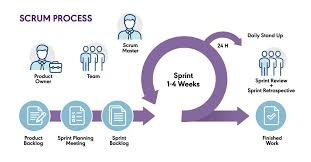
\includegraphics{Image/scrum}
		\caption{Scrum process}
		\label{fig:Scrum process}
	\end{figure}

	\pagebreak
	
	\section{Planning}
	
	\subsection{Forecast Gantt Chart}
	
	\vspace{12pt}
	\begin{figure}[H]
		\begin{ganttchart}[
			x unit=0.8mm,
			y unit chart=7mm,
			time slot format=isodate,
			vgrid={*{30}{white, dashed},*{1}{dotted}},
			]{2024-04-01}{2024-08-31}
			\gantttitlecalendar{year, month=name} \\
			\gantttitlelist{1,...,11}{14} \\ 
			
			\ganttbar{Integration}{2024-04-08}{2024-04-14}\\
			\ganttbar{Application Migration}{2024-04-15}{2024-05-03}\\
			\ganttbar{Employee CRUD}{2024-05-03}{2024-06-14}\\
			\ganttbar{Unit Test}{2024-05-03}{2024-06-15}\\
			\ganttbar{Demonstration}{2024-06-15}{2024-06-15}\\
			\ganttbar{Report}{2024-06-19}{2024-06-21}\\
			\ganttbar{Bug and Improvement}{2024-06-24}{2024-08-09}\\
			\ganttbar{Role Access}{2024-07-1}{2024-08-09}\\
			\ganttbar{Integration Test}{2024-08-01}{2024-08-09}\\
			\ganttbar{CI/CD}{2024-08-07}{2024-08-09}\\
			\ganttbar{Report}{2024-08-12}{2024-08-16}\\
		\end{ganttchart}
		\caption{Forecast Gantt Chart}
		\label{fig:Forecast Gantt}
	\end{figure}
	
	
	\subsection{Actual Gantt Chart}
	\begin{figure}[H]
		\centering
		\begin{ganttchart}[
			x unit=0.8mm,
			y unit chart=7mm,
			time slot format=isodate,
			vgrid={*{30}{white, dashed},*{1}{dotted}},
			]{2024-04-01}{2024-08-31}
			\gantttitlecalendar{year, month=name} \\
			\gantttitlelist{1,...,11}{14} \\ 
			
			\ganttbar{Integration}{2024-04-08}{2024-04-14}\\
			\ganttbar{Application migration}{2024-04-15}{2024-05-08}\\
			\ganttbar{Employee CRUD}{2024-05-08}{2024-06-14}\\
			\ganttbar{Unit Test}{2024-05-03}{2024-06-15}\\
			\ganttbar{Demonstration}{2024-06-24}{2024-06-24}\\
			\ganttbar{Report}{2024-06-19}{2024-06-21}\\
			\ganttbar{Bug and Improvement}{2024-06-24}{2024-08-09}\\
			\ganttbar{Role Access}{2024-07-1}{2024-08-09}\\
			\ganttbar{Integration Test}{2024-08-01}{2024-08-09}\\
			\ganttbar{CI/CD}{2024-08-09}{2024-08-09}\\
			\ganttbar{Report}{2024-08-12}{2024-08-16}\\
			\ganttbar{Project management}{2024-06-15}{2024-08-30}\\
		\end{ganttchart}
		\caption{Actual Gantt Chart}
		\label{fig:Actual Gantt}
	\end{figure}
	\pagebreak
	
	\subsection{Teams}
	
	To manage the tasks and make the collaboration easier, we used Microsoft Teams.\\
	This is a global software that has been useful for a the whole life-cycle of the project. It provides meeting planning, scheduling, Kanban board and collaborative chat.
	
	\begin{figure}[h!]
		\centering
		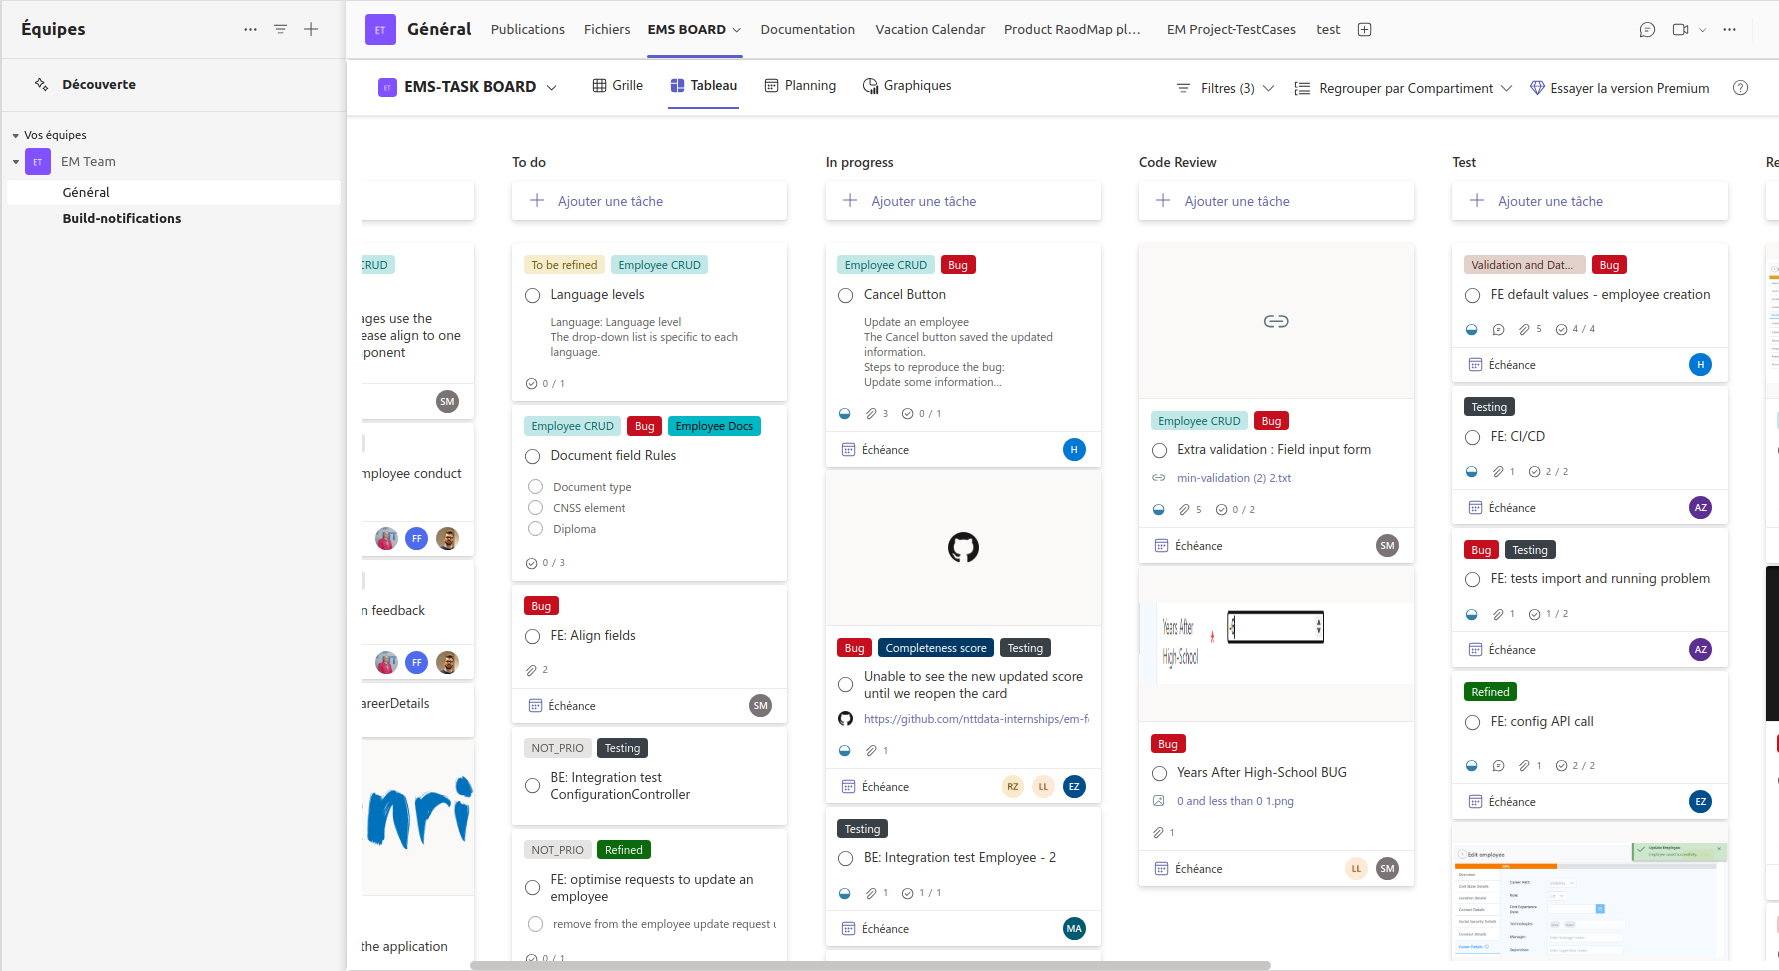
\includegraphics[width=0.8\linewidth]{Image/teams}
		\caption{Teams Kanban Board}
		\label{fig:Teams Kanban Board}
	\end{figure}
	
	\subsection{Github}
	
	Once a task is done, we used Github in order to make Pull Request (PR*). This one is an extension of Git that provide a user-friendly and efficient interface to manage and pinpoint the changes that we want to bring into the project.
	
	\begin{figure}[h!]
		\centering
		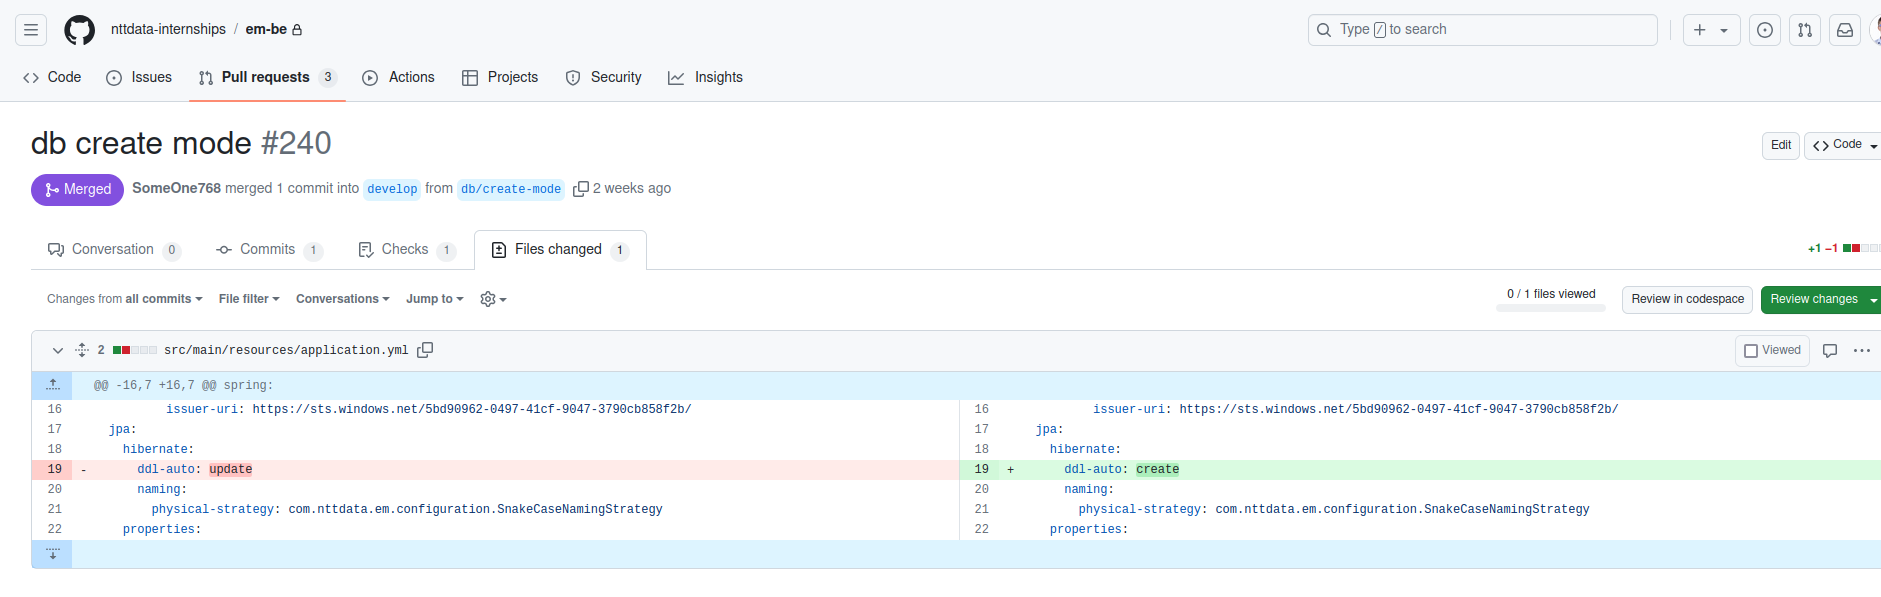
\includegraphics[width=0.8\linewidth]{Image/github}
		\caption{Teams Kanban Board}
		\label{fig:Teams Kanban Board}
	\end{figure}
	\pagebreak
	
	
	\section{Context}

	\subsection{Company presentation}
	
	NTT DATA is a global company providing IT services and consulting, part of the NTT Group (Nippon Telegraph and Telephone Corporation), one of the largest telecommunications conglomerates in the world. Founded in Japan in 1967, NTT DATA offers a comprehensive range of IT services and technological solutions to clients worldwide.\\
	
	As an IT service provider, NTT DATA offers strategy consulting services, application development services, system integration services, IT infrastructure services, business process management (BPM) services, business process outsourcing (BPO) services, and technology infrastructure management services. They work with companies from various sectors, including finance, healthcare, telecommunications, utilities, automotive, and many others.\\
	
	NTT DATA is recognized for its technical expertise, innovation capabilities, and commitment to providing customized solutions that meet the specific needs of its clients. The company leverages emerging technologies such as artificial intelligence, data analytics, the Internet of Things (IoT), and cloud computing to help its clients improve operational efficiency, innovate, and remain competitive in the market.
	
	\begin{figure}[h!]
		\centering
		
\includegraphics[width=0.8\linewidth]{Image/nttgloballogo.png}
		\caption{NTT DATA Logo}
		\label{fig:NTT DATA Logo}
	\end{figure}
	\pagebreak
	
	\subsection{Company historic}
	
	Before delving into the detailed history of NTT DATA, it is worth noting that the company has experienced significant growth and evolution since its establishment in 1967. From its humble beginnings as a subsidiary of NTT, NTT DATA has grown into a leading global company in the IT services and consulting sector. Here is a summary of the key milestones in its historical journey:
	
	\begin{figure}[h!]
		\centering
		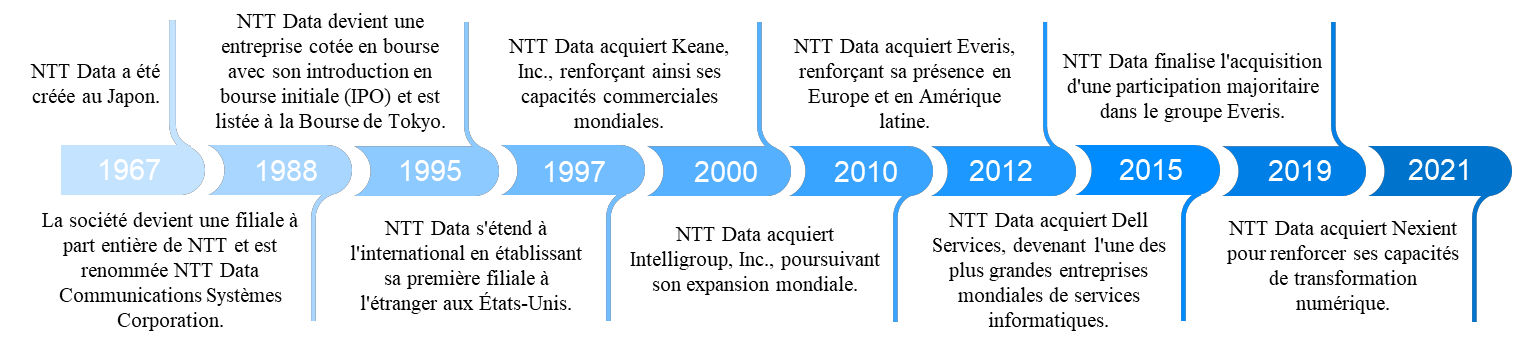
\includegraphics[width=0.8\linewidth]{Image/ntthistoric.png}
		\caption{NTT DATA historic}
		\label{fig:NTT DATA historic}
	\end{figure}
	
	Today, NTT DATA is recognized as one of the global leaders in IT services and consulting, providing innovative technological solutions to its clients worldwide.
	
	\subsection{Global presence}
	NTT DATA has a broad global presence with offices and service delivery centers in many countries around the world.
	\begin{figure}[h!]
		\centering
		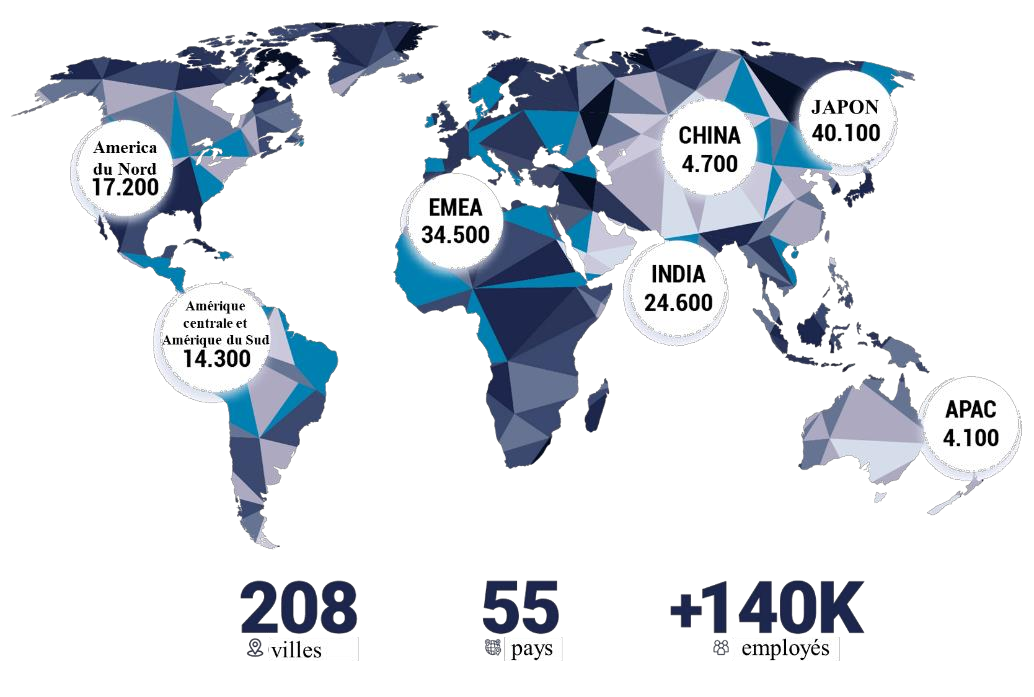
\includegraphics[width=0.8\linewidth]{Image/nttmap.png}
		\caption{NTT DATA historic}
		\label{fig:NTT DATA historic}
	\end{figure}
	
	\pagebreak
	\subsection{Company sector activities}
	
	NTT DATA collaborates with various industries, providing tailored IT solutions and consulting services to address specific challenges and enhance operational efficiency. Here are some key sectors in which NTT DATA is actively involved:
	
	\begin{itemize}
		\item Financial Services: NTT DATA works with financial institutions, banks, insurance companies, and other financial sector players to deliver IT solutions and consulting services aimed at improving operational efficiency, risk management, customer experience, and regulatory compliance.
		
		\item Healthcare and Life Sciences: NTT DATA offers technological solutions to healthcare providers, pharmaceutical companies, and medical research organizations. This includes electronic medical record management, healthcare management systems, health data analytics, tele-medicine services, and clinical trial monitoring solutions.
		
		\item Public Sector: NTT DATA collaborates closely with governments and public sector organizations to provide IT solutions and consulting services that enhance public service delivery, data management, public safety, resource management, and administrative efficiency.
		
		\item Manufacturing and Automotive: NTT DATA provides technological solutions to manufacturers and automotive companies to optimize manufacturing operations, improve supply chain management, integrate the Internet of Things (IoT) into production processes, and develop smart mobility solutions.
		
		\item Telecommunications and Media: NTT DATA partners with telecommunications service providers and media companies to deliver IT infrastructure solutions, digital transformation services, data analytics solutions, online service platforms, and customer management solutions.
		
		\item In addition to these specific sectors, NTT DATA also works with businesses across various industries such as energy, transportation, retail, travel, and hospitality, providing customized IT services and solutions tailored to their specific needs.
	\end{itemize}
	
	\begin{figure}[h!]
		\centering
		
\includegraphics[width=0.8\linewidth]{Image/nttsector.png}
		\caption{NTT DATA sectors}
		\label{fig:NTT DATA sectors}
	\end{figure}
	
	\pagebreak
	
	\subsection{Company services}
	
	NTT DATA, as a trusted global provider of IT services, offers a comprehensive range of services to assist businesses in tackling digital challenges and fostering innovation. The following figure illustrates the services provided by NTT DATA:
	\begin{figure}[h!]
		\centering
		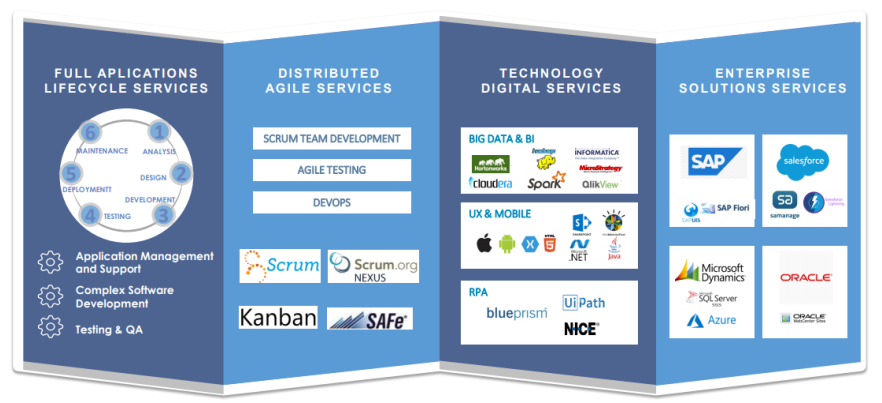
\includegraphics[width=0.8\linewidth]{Image/nttactivities.png}
		\caption{NTT DATA activities}
		\label{fig:NTT DATA activities}
	\end{figure}
	
	\subsection{Partners}
	
	NTT DATA has established strategic partnerships with numerous leading technology and service companies. These partnerships are essential for enhancing NTT DATA's solution offerings and providing added value to its clients. Key partners include industry giants such as Microsoft, Oracle, SAP, Salesforce, IBM, and Amazon Web Services (AWS). These partnerships enable NTT DATA to access the latest technologies and deliver innovative solutions in areas such as cloud computing, enterprise software, customer relationship management, data analytics, and more. Through these strategic partnerships, NTT DATA can offer consulting, integration, and solution management services based on the platforms and technologies of its partners, thereby meeting the diverse needs of its clients across various industries.
	
	
	\begin{figure}[h!]
		\centering
		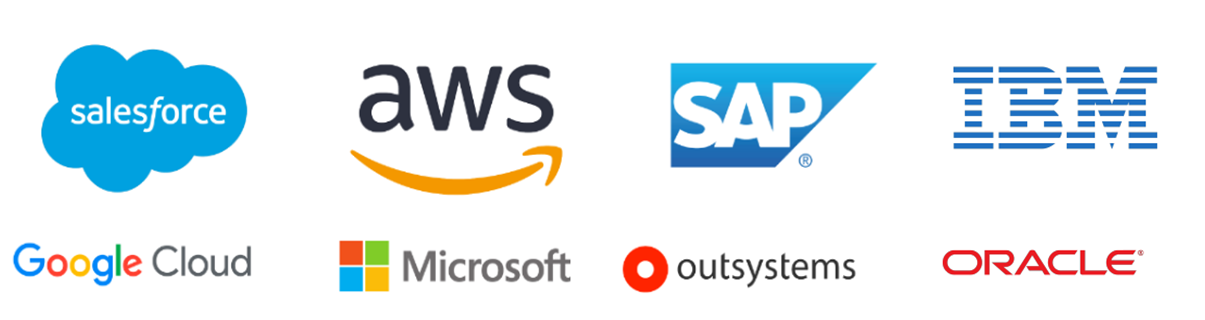
\includegraphics[width=0.8\linewidth]{Image/nttpartners.png}
		\caption{NTT DATA partners}
		\label{fig:NTT DATA partners}
	\end{figure}
	
	\pagebreak
	\subsection{Clients}
	
	NTT DATA's clients encompass a wide range of businesses and organizations worldwide. Leveraging its technological expertise and innovative solutions, NTT DATA has forged lasting partnerships with clients across various sectors including finance, telecommunications, healthcare, manufacturing, and more. Whether serving multinational corporations or local enterprises, NTT DATA is committed to delivering high-quality services tailored to the specific needs of each client. The primary goal is to establish long-term trust-based relationships and contribute to the success and growth of its clients. Here are some of NTT DATA's key clients:
	
	
	\begin{figure}[h!]
		\centering
		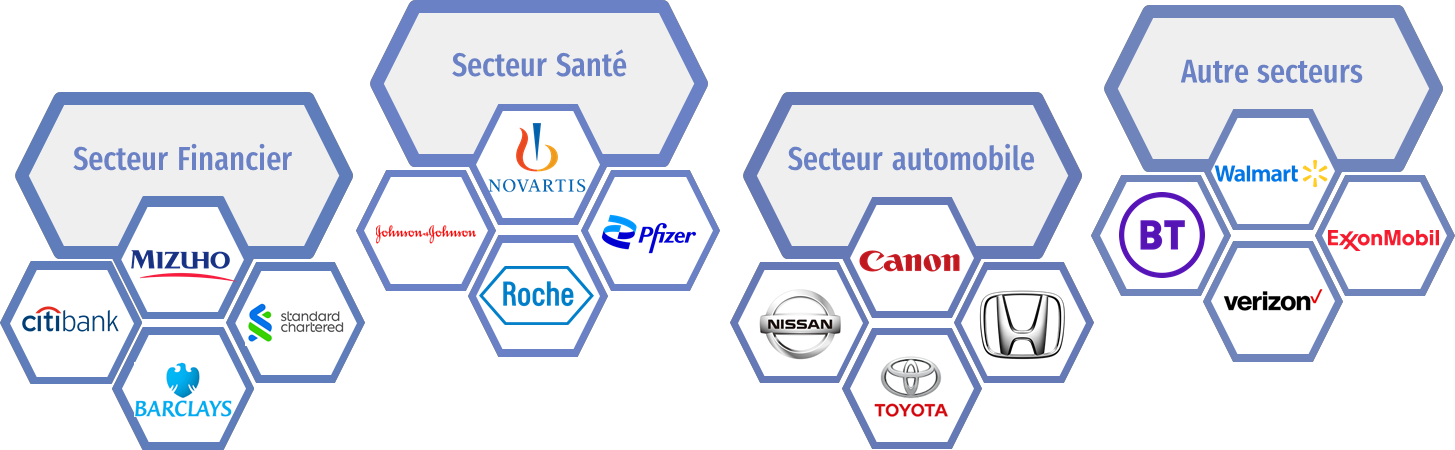
\includegraphics[width=0.8\linewidth]{Image/nttclients.png}
		\caption{NTT DATA clients}
		\label{fig:NTT DATA clients}
	\end{figure}
	
	
	\subsection{Technologies}
	
	
	NTT DATA employs a wide array of technologies to execute and evolve application services for its clients. Among the key technologies utilized are Java, .NET, SQL, Cobol, testing (software testing), and Robotic Process Automation (RPA). These technologies are implemented by a highly skilled and talented team specialized not only in technical aspects but also in industry knowledge. By combining these cutting-edge technologies with deep industry expertise, NTT DATA is able to deliver innovative solutions tailored to the specific needs of its clients, while ensuring high quality and optimal productivity in the execution of their application projects.
	
	\begin{figure}[h!]
		\centering
		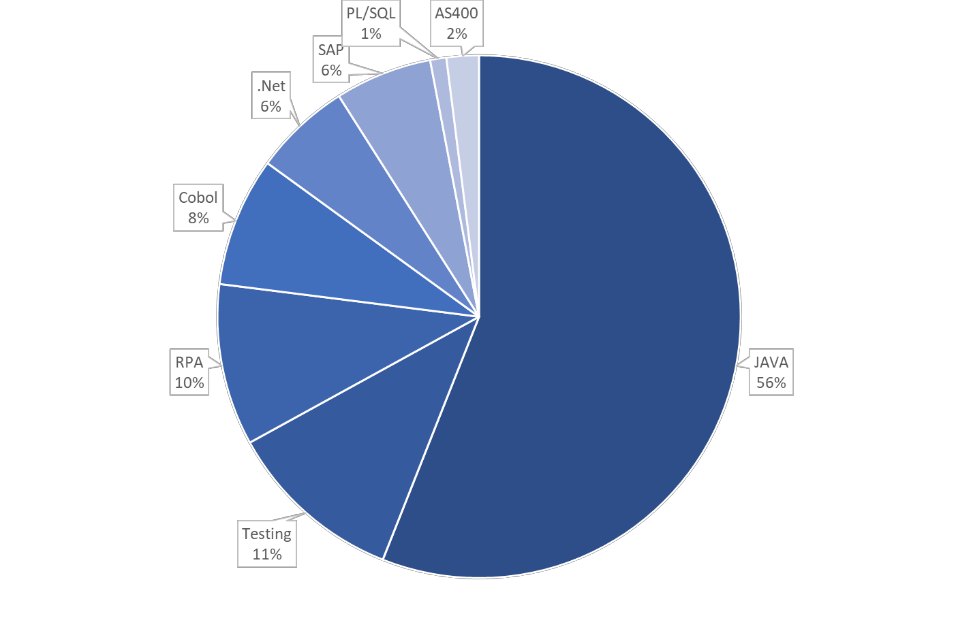
\includegraphics[width=0.65\linewidth]{Image/ntttechnologies.png}
		\caption{NTT DATA technologies}
		\label{fig:NTT DATA technologies}
	\end{figure}
	
	\pagebreak
	
	
	\subsection{NTT DATA in Morocco}
	
	NTT DATA Morocco is a subsidiary of NTT DATA Corporation, a global provider of IT services and technological solutions. The company offers a comprehensive range of services, including software development, IT infrastructure management, technology consulting, digital transformation, and more.\\
	
	NTT DATA Morocco collaborates with local and international clients across various industries such as finance, telecommunications, healthcare, manufacturing, public sector, retail, and other industries. The goal of NTT DATA Morocco is to help businesses optimize their operations, improve efficiency, and address the technological challenges they face.\\
	
	As a subsidiary of NTT DATA Corporation, NTT DATA Morocco benefits from the company's global expertise and experience in the field of information technology. This enables it to offer cutting-edge solutions and innovate in the field of IT services to meet the specific needs of the Moroccan market.\\
	
	NTT DATA Morocco also contributes to the country's technology ecosystem by collaborating with local partners, universities, and institutions to promote innovation, skill development, and growth in the information technology sector in Morocco.
	
	
	\subsection{Career model}
	
	
	NTT DATA employs a career model to enable employees to develop their skills, progress professionally, and achieve their career goals within the company.
	
	\noindent The NTT DATA career model is characterized by the following aspects:
	
	\begin{figure}[H]
		\centering
		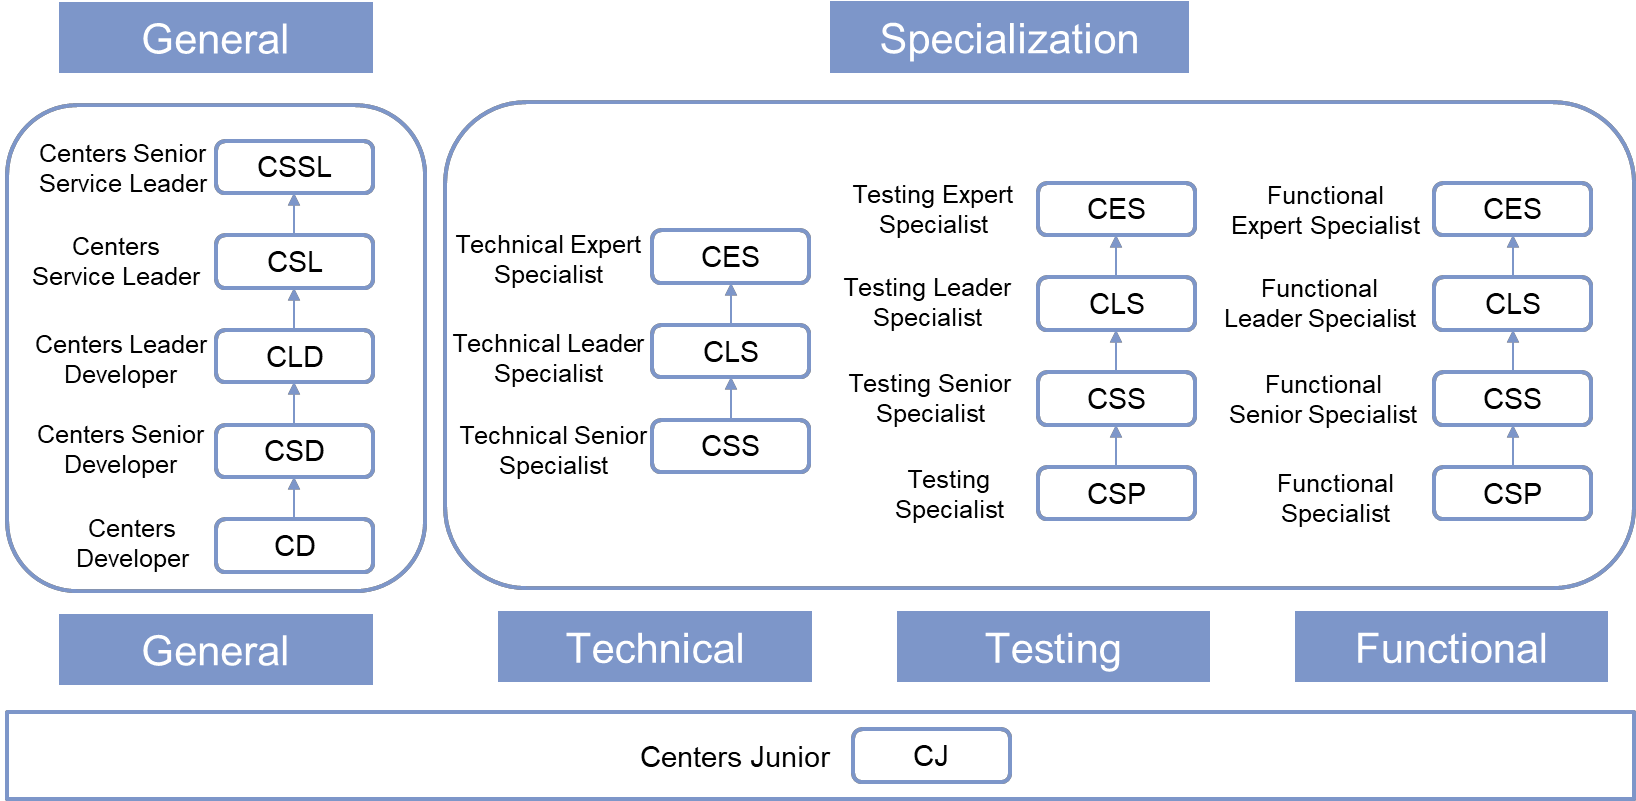
\includegraphics[width=0.65\linewidth]{Image/nttcareer.png}
		\caption{NTT DATA careers}
		\label{fig:NTT DATA careers}
	\end{figure}
	
	\subsection{Societal and environmental responsability}
	
	During the project, we had to keep in mind the need to make an efficient application. This, is not only for performance. Indeed, minimizing and optimizing the application reduces the need of processing and communication between the different services. For this reason, we implemented methods and means at each step and layer of the application in order to streamline resource usage, enhance response times, reduce latency and so reducing our impact on the environment.\\
	
	NTT Data Morocco is also a good place for diversity. This is a multi-cultiral space where different languages are spoken. The official language for the company is english, because of the need to speak with people from different countries but, most of them also speak fluently Spanish in the center of Martil (in addition to Arabic). The center is also a model for gender equality since there as much women and men for the same positions, which is not really common in IT company.
	
	
	\subsection{Problematic}
	
	
	The human resources and staffing workers are using non efficient nor practical way to manage employees and clients of the company.\\
	Using Excel files to store a huge amount of data with the possibility of error and not necessarily normalized practices, this method wasn't maintainable nor evolutive.\\
	
	\noindent The company wants a web application that can help its workers and to manage each one of the processes because currently:
	
	\begin{itemize}
	
		\item Access to employee information is difficult, as it requires manual data searches each time. This leads to time loss and inefficiency in human resource management.
	
		\item Managers must manually organize documents and files related to employees, which can result in document loss and disorganization in tracking information.
	
		\item The absence of an automatic system for generating employee evaluations and promotions, including salary increases and bonuses, makes the process tedious and prone to errors.
	
		\item The lack of a centralized system providing an overall view of the company’s employees, along with all relevant information, as well as a view of the company’s clients and their projects with all associated data, makes the management and monitoring of employees and projects inefficient and fragmented.
	
		\item Management does not have a clear overview of the employees within the company and their status, which can lead to gaps in strategic planning and decision-making.
	
	\end{itemize}


	A fragment of an application had been realized, as a proof of concept (POC*), using \textbf{Elasticsearch} as \textbf{database}* to manage all the data contained in multiple Excel files and this one will be the start of the project.\\
	
	\newpage
	
	
	\section{Analysis and Specifications}
	
	\subsection{Identification and analysis of the needs}
	Currently, the employees and client are managed with Excel files. This method is not efficient and it can lead to many errors in the data itself since it is not normalized. The necessity to create a modern web application to manage the whole life cycle of the employees and clients has become evident. In addition to bring the possibility to have a more efficient and user friendly way to manage the data, it will also be valuable for future data analysis purposes.\\
	
	The principal needs are include the complete management of the clients and the employees information with the possibility to create and manage projects assignment on them.
	
	\begin{figure}[h!]
		\centering
		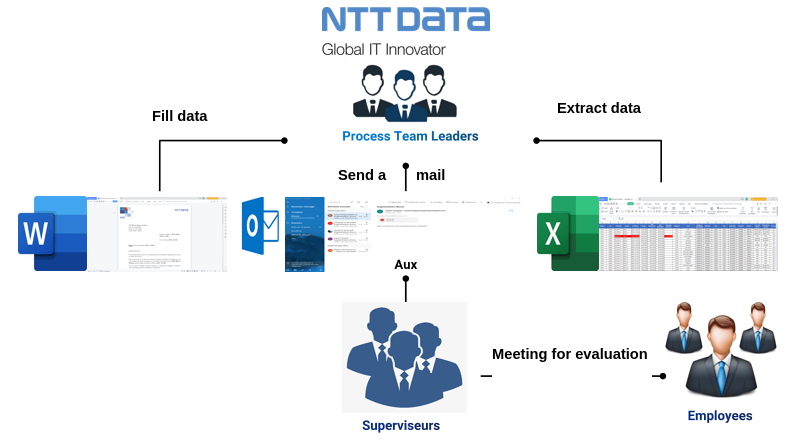
\includegraphics[width=0.65\linewidth]{Image/current_app.png}
		\caption{Current management}
		\label{fig:Current management}
	\end{figure}


	\subsection{Functional specifications}
	\subsubsection{Actors}
	The application is designed to accommodate different types of users, with four main \textcolor{purple}{\textbf{roles}} assigned.\\
	Firstly, the application is divided into two distinct sections:\\
	
	\begin{itemize}
		\item Staffing (\textcolor{purple}{\textbf{staffing}}, \textcolor{purple}{\textbf{manager}})
		\item Human Resources (\textcolor{purple}{\textbf{hr}})
	\end{itemize}

	\noindent Additionally, there is a global role: \textcolor{purple}{\textbf{admin}}. This role is reserved for developers, granting them access to all functionalities for the purposes of enhancing and debugging the application.
	Later, the application should be able to discriminate users based on their hierarchical position.
	\pagebreak
	
	\subsubsection{Main functionalities}
	The main functionalities in our applications are:
	\begin{itemize}		
		\item Employee management: This one allow to have a track about the current state of each employee including his global data (personal, contract, documents ...). It includes not only the creation and the update but also a way to archive since we never really delete anything in the app (except with admin right).
		
		\item Client management: Like the previous ones we have a way to manage the global information of any client.
		
		\item Fetch a list of employees.
		
		\item Search based on criteria (names, position, ID, status, project name) or on a keyword.
		
		\item Project management (including assignments).
		
		\item Promotions management to allow manager to have a track and make evolution easier in the company.
		
		\item Company objectives management.
		
		\item Simulation management that provide a way to create and manage simulations of various scenarios, helping in decision-making.
		
	\end{itemize}


	\newpage
	
	\subsection{Non-Functional specification}
	
	It is necessary to also directly include some specifications that are not directly linked to the needs in order to build an application as clean and efficient as possible.
	
	
	\begin{center}
		\begin{tabular}{| p{3cm} | p{12cm} |}
			\hline
			Requirements & Description \\\hline
		
			Performance & The application should provide fast loading times and smooth user interactions, even under high user load. This includes quick response to user inputs and efficient data processing. \\\hline
		
			Security & The application need to have strong protection measures including authentication, access controls, and encryption to prevent unauthorized access and data leak. \\\hline
		
			Reliability & The application should minimize the error and manage it both by using HTTP errors and revoking changes. \\\hline
		
			Scalability & The application should provide modularity and flexibility, allowing for the addition of new features and seamless integration with other systems or services as the application evolves. This ensures that the application can handle increasing volumes of users and data over time. \\\hline
		
			Maintainability & The application must be easily maintainable and extensible. The code source should be well-organized, documented, and adhere to best development practices to facilitate updates, bug fixes, and future enhancements. \\\hline
			
			Usability & The user interface must be user-friendly, intuitive, and accessible. Users should be able to navigate the application easily, complete their tasks without confusion, and enjoy a pleasant overall experience \\\hline
		\end{tabular}
	\end{center}
	
	
	In addition to, this application should include some dynamic settings. Indeed, it will run into different location and some parameter can also evolve over the time. For this reason, we should be able to change parameters without stopping the application.
	
	
	\section{Modelisation}
	
	After the analysis, we identified the need and started to build the architecture of the application with different diagrams.
	
	\subsection{UML}	
	A huge UML file that couldn't be integrated in this report is available here: \url{https://drive.google.com/file/d/1ERMLGaywMv31-N9RHgPd562t4h1-OXjg/view?usp=sharing}\\
	
	\subsection{Classes}
	\begin{center}
		\renewcommand{\arraystretch}{1.5} % Adjust the row height
		\begin{tabularx}{\textwidth}{| l | X |}
			\hline
			\textbf{Class} & \textbf{Description} \\\hline
			
			AuditableEntity & Class from which all others will inherit to track creation and modification date\\\hline
			
			BankAccountDetails & Represents the bank information of an employee\\\hline
			
			BonusSimulation & Represents bonus simulations \\\hline
			
			CategoryMappings & Represents the hierarchical position of an employee\\\hline
			
			CenterPromotionObjective & Represents the objective for a center\\\hline
			
			CivilStateDetails & Represents the civil information of an employee\\\hline
			
			Client & Represents a client\\\hline
		
			ContractDetails & super class for different contract types\\\hline
		
			EntryLevelContractDetails & Represents the type of contract for people that are still learning (ANAPEC in Morocco) \\\hline
			
			PermanentContractDetails & Represents a permanent contract \\\hline
			
			SubContractorContractDetails & Represents a contract with an external person (Freelancer) \\\hline
		
			Country & Represents a country\\\hline
			
			Cost & Represents the cost associated with an employee or a project \\\hline
			
			Dependent & Represents a person that an employee is in charge of such as children.\\\hline
			
			Document & Represents an upload document such as pictures and hold the link for the Minio server[ici]\\\hline
			
			PromotionObjective & Represents the objective for promotions \\\hline
			
			EducationalDetails & Represents a diploma\\\hline
			
			Employee & Represents the employee \\\hline
			
			Evaluation & Represents the evaluation and feedback given during an interview \\\hline
			
			EvaluationObjective & Represents a specific objective to be assessed during a performance evaluation \\\hline
			
			HeadCountObjective & Represents the staffing objective \\\hline
			
			ImportLog & Store detail about user that are importing data from excel file\\\hline
			
			LanguageProficiencyDetails & Represents a language known by an employee\\\hline
						
			LocationDetails & Represent an address\\\hline
			
			
		\end{tabularx}
	\end{center}


	\begin{center}
		\renewcommand{\arraystretch}{1.5} % Adjust the row height
		\begin{tabularx}{\textwidth}{| l | X |}
			\hline
			\textbf{Class} & \textbf{Description} \\\hline
			
			NetSalary & Represents the monthly salary of an employee \\\hline
						
			Position & Represents the position occupied by an employee \\\hline
			
			Project & Represents the project \\\hline
			
			Promotion & Represents the promotion \\\hline
			
			RuntimeSettings & Represents the dynamic parameters of the application\\\hline
			
			SalaryBand & Represents a salary range with minimum and maximum limits for a position \\\hline
			
			SalaryIncrease & Represents salary increases \\\hline
			
			StaffedRole & Represents the employee's role regarding a project \\\hline
			
			StaffingRecord & Represents an activity performed by an employee related to a project \\\hline\hline
			
			PeopleInterviewFeedback & Related to the promotion cycle\\
			ProductionInterviewFeedback & \\
			TechnicalInterviewFeedback & \\
			TechnicalQuestion & \\
			TechnicalQuestionScore & \\
			Topic & \\\hline
			 
		
		\end{tabularx}
	\end{center}

	\newpage	
	
	\subsection{Sequence diagrams}
	
	We now need to explore the interactions and the processes for the system. For this purpose, we will use sequence diagrams.
	
	\subsubsection{Authentication}
	
		\begin{figure}[H]
		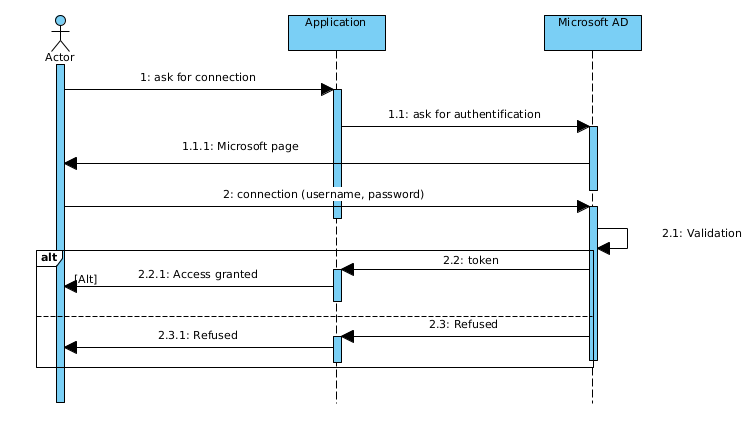
\includegraphics[width=150mm]{Image/seq-authentication}
		\caption{Authentication diagram}
		\label{fig:Authentication diagram}
		\end{figure}
	
	\subsubsection{Creation}
	
	\begin{figure}[H]
		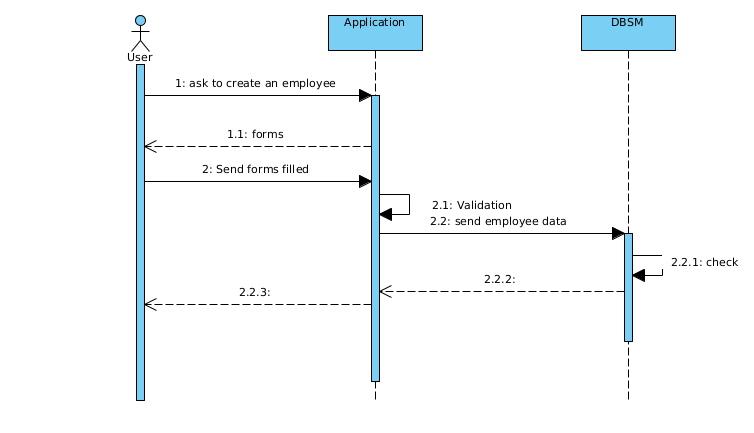
\includegraphics[width=150mm]{Image/seq-createemp}
		\caption{Create employee diagram}
		\label{fig:Create employee diagram}
	\end{figure}
	
	\begin{figure}[H]
		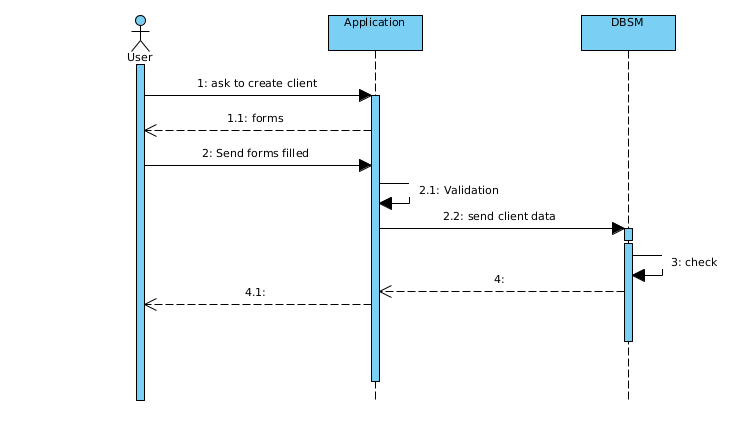
\includegraphics[width=150mm]{Image/seq-createclient}
		\caption{Create client diagram}
		\label{fig:Create client diagram}
	\end{figure}

	\subsubsection{Project assignement}

	\begin{figure}[H]
		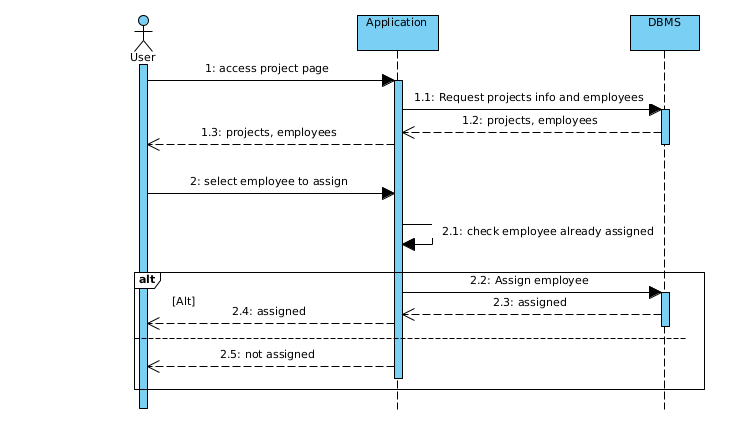
\includegraphics[width=150mm]{Image/seq-assigntoproject}
		\caption{Employee assignment to project diagram}
		\label{fig:Employee assignement to project diagram}
	\end{figure}


	\newpage
		
	\section{Environment}
	
	\subsection{Physical architecture}
	
	The physical architecture is distributed across several services, each running on its own server. The services are designed to be scalable, allowing the system to handle increased load by adding more instances as necessary, using AWS cloud computing.
	
	\subsubsection{Model-View-Controller Architecture}
	
	The Model–view–controller (\textbf{MVC}*) is a software design pattern* which goal is to enhance the modularity, maintainability, and scalability of our system. It separates the application into three distinct layers, components:
	
	\begin{enumerate}
		\item The \textbf{model} which is the representation of the information and represented by the Database;
		\item The \textbf{view} which is the presentation layer that display the information and interact with the user;
		\item The \textbf{controller} which is the link between the 2 previous one but also the processing layer.
	\end{enumerate}
	
	\begin{figure}[H]
		\centering
		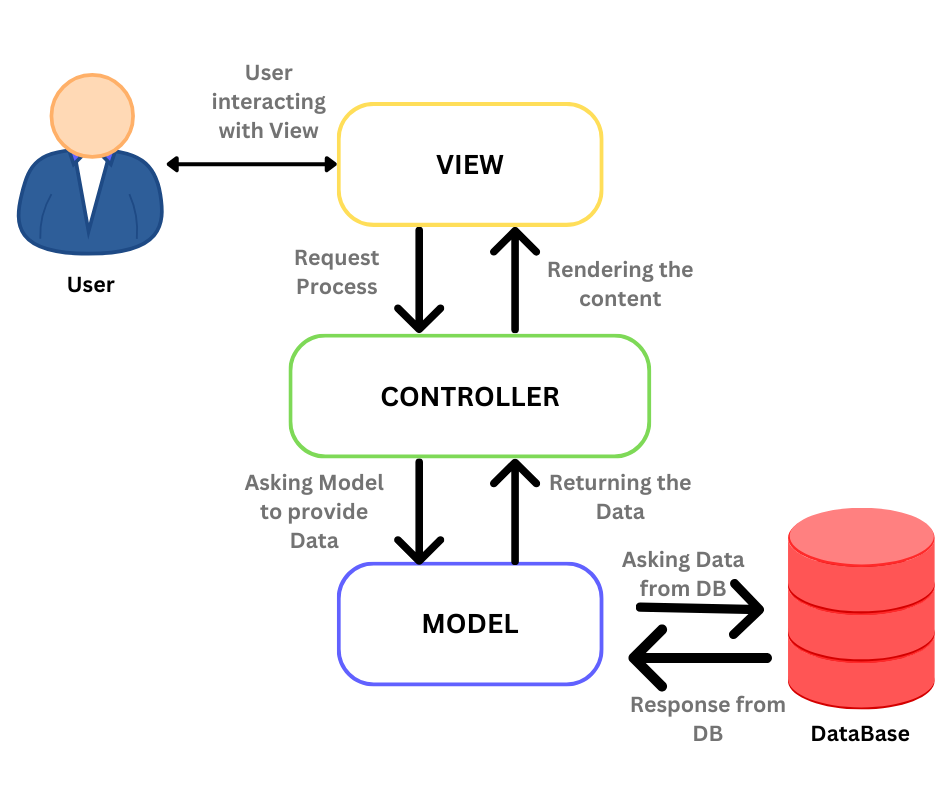
\includegraphics[width=150mm]{Image/mvc}
		\caption{MVC architecture}
		\label{fig:MVC architecture}
	\end{figure}
	
	\pagebreak
	\subsection{Software architecture}
	
	\subsubsection{Back-End}
	%A new architecture has been conceived to accommodate the expanded scope of the project. Unlike the previous iteration, which focused primarily on basic employee information management such as names, email addresses, and phone numbers, the revised architecture will encompass a broader range of functionalities. This expanded scope includes the capability to create and manage contracts, as well as managing all the projects within the organization.
	
	The back-end server is responsible for managing business operations and processing data. It plays a crucial role in linking the database with the user ensuring that data flows seamlessly between him and the system. To ensure smooth and efficient communication, an appropriate architecture is essential. In our case, we have chosen to use a RESTful API which is known for its scalability, flexibility and ease of integration with various client applications.\\
	
	\noindent The back-end has been implemented using a layered design model. This one divide the server into multiple layer where each one is responsible for specific task: 
	
	\begin{itemize}
		\item \textbf{Controllers}: act as the entry point for user requests. They handle incoming HTTP requests, extract necessary parameters, invoke the appropriate services, and return the results in the form of HTTP responses.

		
		\item \textbf{Services}: contains the core business logic. It processes the data according to the business rules and coordinates with the repository layer to retrieve or update data in the database. This layer encapsulates complex operations, making it reusable and maintainable
		
		 
		\item \textbf{Entities}: representation of the object stored inside the database which is complete and linked to all other entities present in the UML.
		
		\item \textbf{Data Transfer Object (DTO*)}: they are used to transfer the data, minimized and filtered, for communication between the server and users.
		 
		\item \textbf{Mappers}: those ones can be seen as converters that transform entities to DTO and DTO to entities. In our case, those ones are also useful for updating entities based on new changes made on DTO.
		
		\item \textbf{Repository}: responsible for data access and persistence, it give us all the necessary operations to communicate with the database.
		
	\end{itemize}

	\begin{figure}[H]
		\centering
		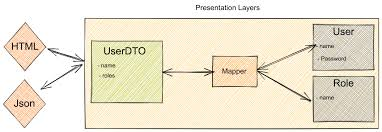
\includegraphics[width=150mm]{Image/dto}
		\caption{DTO exemple}
		\label{fig:DTO exemple}
	\end{figure}	
	
	\newpage
	\subsubsection{Front-End}
		
	The front-end is the client side of the application which provide the user interface. This one manages how the data will be displayed and how the user will be able to interact with the back-end server while ensuring a smooth navigation between the different resources. \\
	
	\noindent The Front-End uses a component architecture. This allows us to develop and use small and reusable code through the user interface using component. Each one contains both the presentation and the logic that will be applied.
	
	\begin{itemize}
		\item \textbf{Component:} it is a piece of the user interface that contains its own HTML* (presentation), CSS* (style) and TS* (logic)
		
		\item \textbf{Module:} container that regroup different components, directives, services and functionalities.
		
		\item \textbf{Service:} class that provides shared functionality that can be used in different part of our application. It contains specifically the part of the code that handles the request with the back-end server.
		
		\item \textbf{Directive:} allows to dynamically interact and manipulate the DOM*. %exemple pour les validators; [input]...
		
		\item \textbf{Template:} HTML file that define the appearance of components
	\end{itemize}

	\newpage
	
	\subsection{Technologies}
	
	\subsubsection{Back-End}
	
	Java programming language has been chosen to develop the Back-End. It includes different frameworks that not only help us to facilitate the development but also structuring it into multiple layers, each one with a specific responsibility.
	
	We have also included multiple frameworks and libraries to enhance performances, and maintain clean and modular code.\\
	
	\paragraph{Spring Boot:} this is the core of our application. Spring boot is the most used Java framework that will provide a lot of features for the different layers of the application. It helps for auto configuration, deploying execution environments but also managing dependencies injections.
	
		
	\begin{figure}[H]
		\centering
		
\includegraphics[width=70mm]{Image/springboot}
		\caption{Spring Boot Framework}
		\label{fig:Spring Boot Framework}
	\end{figure}
	
	
	\paragraph{Spring Security:} providing strong security features to easily manage sessions, authentication and authorization. This one help to protect the resources of the application.
	
	\begin{figure}[H]
		\centering
		
\includegraphics[width=70mm]{Image/springsecurity}
		\caption{Spring Security Framework}
		\label{fig:Spring Security Framework}
	\end{figure}
	
	\paragraph{Spring Data JPA and Hibernate:} technologies that facilitate the communication with database. While JPA provide all the basic functions \citep{JPA2, JPA1} to access, modify, retrieve and delete the data from the database, Hibernate allow us to map Java objects to database tables, managing the complex relationships between the entities. It also optimize the performances using cache and lazy-loading. Finally, if we want more, we can make native SQL query \citep{JPA3} for more complex usage.
	
	\begin{figure}[H]
	\centering
	
\includegraphics[width=70mm]{Image/springdata}
	\caption{Spring Data Framework}
	\label{fig:Spring Data Framework}
	\end{figure}
	
	\paragraph{Spring Test:} testing framework that provide tools to support unit and integration testing for the applications. It simplifies the process of writing and executing tests by allowing the injection of dependencies, management of application contexts, and configuration of mock* environments. Finally, we can easily set up tests that will use the same configuration and beans* as our production environment.
	
		
	\begin{figure}[H]
		\centering
		
\includegraphics[width=70mm]{Image/springtest}
		\caption{Spring Test Framework}
		\label{fig:Spring Test Framework}
	\end{figure}

	\paragraph{Annotations:} it simplifies the code by providing features, generated code and behavior to components such as controllers, services or repositories by just writing small words preceded by '@'.
	
	
	\subsubsection{Front-End}

	The Front-End of our application is developed with Angular, a popular and powerful framework that provides a lot of tools and features that streamline the development process, ensuring a responsive and efficient user interface. It allow us to build dynamic, single-page applications (SPAs), that avoid the user to reload the whole page when he navigates and instead just reload the necessary resources.
	
	
	\paragraph{Angular Framework:}
	Built on TypeScript, it offers a modular architecture using reusable components, services, and modules. This modularity helps in maintaining a clean and organized code base, making it easier to manage and scale the application as it grows. Angular’s component-based structure promotes re-usability and separation of concerns, ensuring that each part of the UI is independent and can be developed and tested in isolation.
	
			
	\begin{figure}[H]
		\centering
		
\includegraphics[width=70mm]{Image/angular}
		\caption{Angular Framework}
		\label{fig:Angular Framework}
	\end{figure}
	\newpage
	\paragraph{Data Binding:}
	Angular supports two-way data binding, which automatically synchronizes data between the model and the view. This feature reduces the amount of boilerplate code required to update the UI in response to user input or changes in the underlying data, leading to a more responsive and interactive user experience.
	
	\paragraph{Forms and Validation:}
	Angular provides powerful tools for creating and managing forms, including support for both template-driven and reactive forms. With Angular's validation features, we can easily implement client-side validation to ensure data integrity and provide immediate feedback to users, improving the overall user experience.
	
	\paragraph{HTTP Client:}
	Angular’s HTTP client module simplifies communication with the back-end RESTful API. It provides a straightforward API for sending HTTP requests and handling responses, including error handling and interceptors for adding common headers or managing authentication tokens.
	
	\paragraph{Style:}
	Angular includes styling libraries and frameworks such as PrimeNG, which has been integrated in our application. It is a UI* component's library that provides a wide collection for useful component such as button, array or calendar.\\
	
	\begin{figure}[H]
		\centering
		
\includegraphics[width=60mm]{Image/primeNG}
		\caption{primeNG logo}
		\label{fig:primeNG logo}
	\end{figure}
	
	\noindent The languages that are being used to develop our Angular application are:
	
	\paragraph{TypeScript:} developed by Microsoft, it adds static typing to the JavaScript language. It helps to organize the code and allows to detect the error at the compilation.
	
	\paragraph{JavaScript:} this language is responsible for the management of dynamic behaviors, events, DOM manipulations, requests and a lot of others functionalities in the client side.
	
	\paragraph{CSS:} it is used to for the styling of the presentation layer. CSS is responsible for the color, the police, positioning, size ...
	
	\paragraph{SQL:} SQL is the most basic language used to communicate with the database. It allows to manipulate and manage the relational data by stocking, fetching, updating, deleting the data. It guarantee data integrity and is widely supported by various DBMS.
	
	\paragraph{HTML:} ballistic languages, it provides a structure for the layer presentation. 

	\subsubsection{Database}
	
	The initial database management system (DBMS*) of the application was Elastic search*, a powerful search engine designed for handling large volumes of data. This one is mostly useful for analytics while we were more looking for something more traditional that will manage structured data. For this reason we moved for PostgreSQL. It is an open source DBMS, among the most popular \citep{stat1, stat2}, that extend the SQL language by adding advanced features such as procedures, triggers and functions. It is widely used in the web development and other applications that require reliable and high-performance data storage.
	
	
	\subsection{Developing tools}
	
	Additionally to the programming languages, frameworks*, libraries* that are being used, we also use some other softwares that help us in the whole development cycle.
	
	\paragraph{Maven:} popular tools that automate the management of the dependencies*, mostly used for java projects. It provides a standardized way to manage project dependencies, compile source code, run tests, package applications, and deploy them across various environments including CI/CD*. 
	
	\paragraph{Node.js:} Node.js is a server-side JavaScript runtime environment that enables the development of high-performance and scalable web applications. It uses an event-driven, non-blocking architecture, making it ideal for handling many simultaneous requests. Thanks to its rich ecosystem and growing popularity, Node.js has become one of the preferred choice for developing fast and efficient applications.
	
	\paragraph{Node Package Manager (npm):} npm is the package management tool for Node.js. It allows developers to install, share, and manage libraries and dependencies for their JavaScript projects efficiently. 
	
	\paragraph{Swagger:} Swagger is a suite of tools for designing, building, and documenting API* efficiently. It facilitates the creation of interactive and accurate documentation while providing automated features for validating and testing endpoints. Swagger promotes collaboration between development and documentation teams and enhances API interoperability.
	
	
	\paragraph{Visual Studio Code:} Visual Studio Code is a lightweight yet powerful IDE developed by Microsoft. It provides a user-friendly interface and a wide range of features to facilitate software development for several languages. VS Code supports numerous programming languages and offers capabilities such as syntax highlighting, auto-completion, debugging, integrated version control, and integration with popular tools and extensions.
	
	\paragraph{IntelliJ IDEA:} IntelliJ IDEA is a powerful and versatile IDE developed by JetBrains. Widely used for Java software development, it offers advanced features such as intelligent code editing, debugging, refactoring, dependency management, and more. It is popular among developers for its ease of use, performance, and support for major frameworks and development technologies.
	
	
	\paragraph{Git and GitHub:} it is a distributed version control system that allows for the management of different versions of source code. GitHub is a platform built on Git that facilitates collaboration and project management. We have used Git and GitHub to ensure source code traceability and to streamline the development process by enabling separate development of each component, thereby reducing complexity. In addition to, Github allows users to make Pull Request, which is an efficient and user friendly way to propose the adding of code to the main branch*. 
	
	
	\subsection{Different servers and services}
	
	We have multiples servers that we can manage through Heroku*, hosted in Amazon Web Service (AWS*) cloud. They include not only the back-end and front-end servers but also several other services that enhance the application's functionality.
	
	\begin{itemize}
		\item \textbf{Java Back-End Server:} server that handles the business logic, API requests, and interactions with the database representing the controller layer.
		
		\item \textbf{Angular Front-End Server:} server that hosts the Angular-based front-end, which is responsible for rendering the user interface and handling client-side logic. It serves the view layer, ensuring that users have a responsive and interactive experience.
		
		\item \textbf{PostgreSQL Database Server:} server that manages the PostgreSQL database, which serves as the model layer. It stores all the application data.
		
		\item \textbf{Minio Server:} server that is used for storing complex and heavy data such as files or images.
		
		\item \textbf{Azure Active Directory:} we integrated Azure Active Directory for authentication and authorization processes. This service handles user identity management, providing secure access control and ensuring that only authorized users can access the application. It also allows to provide role for specific parts of the application thanks to the role management.
		
	\end{itemize}

	
	%\subsection{Technologies}
	
	%\subsubsection{Back-end}
	
	%The language Java has been chosen for our application. Firstly because the previous application was already made with but also because it is known for its portability across different operating systems, Java enables our applications to run seamlessly in diverse environments without making any adjustment, which is particularly usefull as developpers use as well Windows, Mac and Linux. Its strong typing and object-oriented features help ensure code reliability and maintainability.\\
	
	%Additionally, Java includes a lot of libraries and frameworks that accelerates development and allows us to integrate a variety of efficient functionalities. More specifically, we are using Spring Boot [TODO]. This last one is an open-source framework that simplifies the development of our applications by providing a comprehensive set of features and tools. Spring Boot enables developers to implement commons functions [TODO mapstruct] and manage dependancy injection [TODO].
	
	\newpage
	
	\section{Security}

	As we previously said, AD is part of the security chain. Indeed, in modern web applications, token-based authentication are really common and efficient method to ensure secure communication between clients and servers. A \textbf{token}* is a digital key used to authenticate users and validate their access to resources or services. Unlike traditional session-based authentication, where the server holds session data, token-based authentication relies on stateless communication, meaning the server does not need to store information about the user between requests. This is a great advantages when we have a multi-services application and when a lot of user are using the application as we can redirect to any of them without needing to authenticate again (especially because it is a stateless method).\\
	However, in our application, this is not enough.
	
	\subsection{Role Access Management}
	The application is a fusion of two distinct projects that share common code. Each project includes functionalities tailored for two different roles: staffing and HR. Therefore, we need to secure our API not only with authentication but also based on the role of the current user. Additionally, some functionalities are also restricted to privileged users such as managers or admins. 
	
	
	\subsubsection{Open Policy Agent}
	
	Open Policy Agent (OPA)*\citep{OPA} is an open-source solution that enables us to define, enforce, and manage policies for our systems and services. OPA is designed to be flexible and high-performance, with minimal processing requirements (RAM, CPU ...), allowing easy integration into different environments and independence from the programming language used. 
	
	
	\paragraph{Deployment}: OPA needs to run as a separate service or server. This requires deploying a new server in the cloud, though OPA's lightweight processing footprint ensures it remains almost invisible in terms of resource consumption and so it is a waste of money for our use case as we would be force to deploy a new server. It could also be installed using Docker* but this is currently not possible in our platform. Another solution would be to have a standalone binary that can be run directly inside our application. However this last one requires to allow command execution* and is dependent on the OS* used, this make it not possible for us. 
	
	\pagebreak
	
	\paragraph{Functionning}: Once deployed, OPA controls access using a list of rules written in Rego, its declarative policy language. These rules are evaluated to make policy decisions, enabling fine-grained access control across various services and systems. OPA evaluates incoming requests against these rules and returns a decision, ensuring that access is granted or denied based on predefined policies. 
	
	
	\paragraph{Integration}: To integrate OPA, after running it as another service we will communicate with thanks to request where we can send anything as JSON* for our rules. For this, in our spring boot application we use filters* that will handle all the requests and redirect it into OPA. Based on the return it will give, will either pursue the processing of the request or denied the access of the end point to the user. 
	
	\begin{figure}[H]
		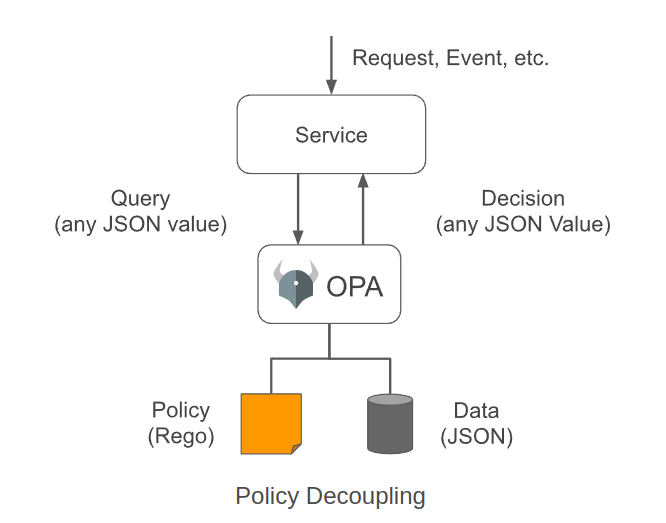
\includegraphics[width=150mm]{Image/OPA}
		\caption{OPA deployment}
		\label{fig:OPA deployment}
	\end{figure}
	
	\pagebreak
	\subsubsection{Cache management}
	
	Another approach has been explored and then chosen. Instead of deploying complex services and using special policies* we can indeed build a table that will contains our rules. This one is more efficient as it is accessible directly in the application and need no communication.
	
	\begin{center}
		\begin{tabular}{| c | c | c |}
			\hline
			method & end point & roles allowed\\ \hline
			GET & /employees/\{id\} & HR, STAFFING\\
			\hline
		\end{tabular}
	\end{center}
	
	\noindent Since access needs to be checked for each request, processing can become intensive for this simple task. To optimize these access checks, we can use a caching mechanism that reduces the computational loading for evaluating access decisions by storing the table directly in the cache. This one enhances the performance by quickly serving subsequent requests.\\
	Indeed, we can manage the cache to improve it again. 
	Instead of caching the entire table and searching through it for access control decisions, we can optimize both space and processing by caching the results of the function itself. With a well-structured approach, we can store the function's output based on its parameters. By using a long expiration policy, we reduce the need to reprocess this function frequently. Once the function has run and its result is cached, subsequent requests with the same parameters can retrieve the result directly from the cache, eliminating the need to evaluate the function again.
	
	
	\paragraph{Deployment}: the cache is directly managed inside the application, we don't need to do anything else than configuring the name, the type that will be stored and a unique key to access each element. Finally the time to leave is also configurable. 
	
	
	\paragraph{Functionning}: Usually, the cache is used to store complex objects to avoid redundant computations and expensive operations. By caching these complex objects, we reduce the need for recalculating or re-fetching data, which enhances performance and efficiency.  
	In our case, the cache helps by directly storing access check results. Indeed we have a long list where we need to check if a role has the access to a certain end point. Searching in this list at each request may be not efficient and not interesting for us. For this reason, we directly cache the result of a function that will search inside this list. Whenever we try again with the same parameters, instead of looking inside this list the cache will directly give us the answer. 
	
	
	\paragraph{Integration}: To integrate this caching-based access management method, we use a filter* that intercepts requests after authentication. This filter extracts user information, including the current role, from the authentication token. Based on the user's role and the requested endpoint, the filter checks the access permissions stored in the cache. This allows the system to efficiently determine whether to grant or deny access to the requested end point. 
	
	\newpage
	
	\section{Tests}
	
	Testing is a critical phase in software development. It aims to ensure the quality, reliability, and robustness of the code but also helps in identifying errors, bugs, and potential issues before the software is deployed to production. There are various types of tests, each serving a specific purpose within the software development life-cycle. Unit tests and integration tests\citep{TESTBD, TESTOC} are among the most common approaches, each playing a vital role in maintaining software quality and are the 2 currently implemented in the application.\\
	Testing also allow us to maintain the application by ensuring that there is no regression. Indeed, sometimes by adding a functionality or modifying the code we may break the application or add a bug.
	
	
	\subsection{Unit Tests}
	Unit tests focus on verifying the functionality of individual components or pure functions. These tests are designed to ensure that each piece of code behaves as expected under various conditions. Unit tests are typically written and run by developers during the development process to catch errors early and maintain code quality. By testing the smallest units of code independently, unit tests provide a strong foundation for reliable software.
	
	\subsection{Integration Tests}
	Integration tests evaluate the interaction between multiple components or systems to ensure they work together as intended. These tests are crucial for identifying issues that may arise when different parts of the application are combined. Integration tests can involve testing the interaction between modules, services, or external API. By simulating real-world scenarios, integration tests help ensure that the entire system functions cohesively and meets the desired requirements.
	
	\newpage
	
	\section{Application}
	
	\subsection{Authentication}
	Whenever the user want to access the application he is first redirected to the connection page
	
	\begin{figure}[H]
		\centering
		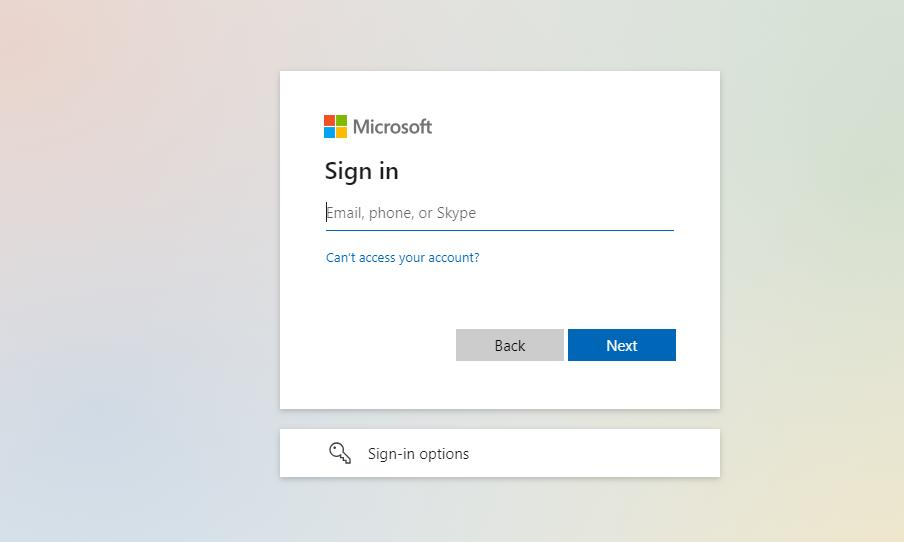
\includegraphics[width=150mm]{Image/authentication}
		\caption{Authentication page}
		\label{fig:Authentication page}
	\end{figure}


	\subsection{Dashboard}
	A dashboard is present to display information about the employees
	
	\begin{figure}[H]
		\centering
		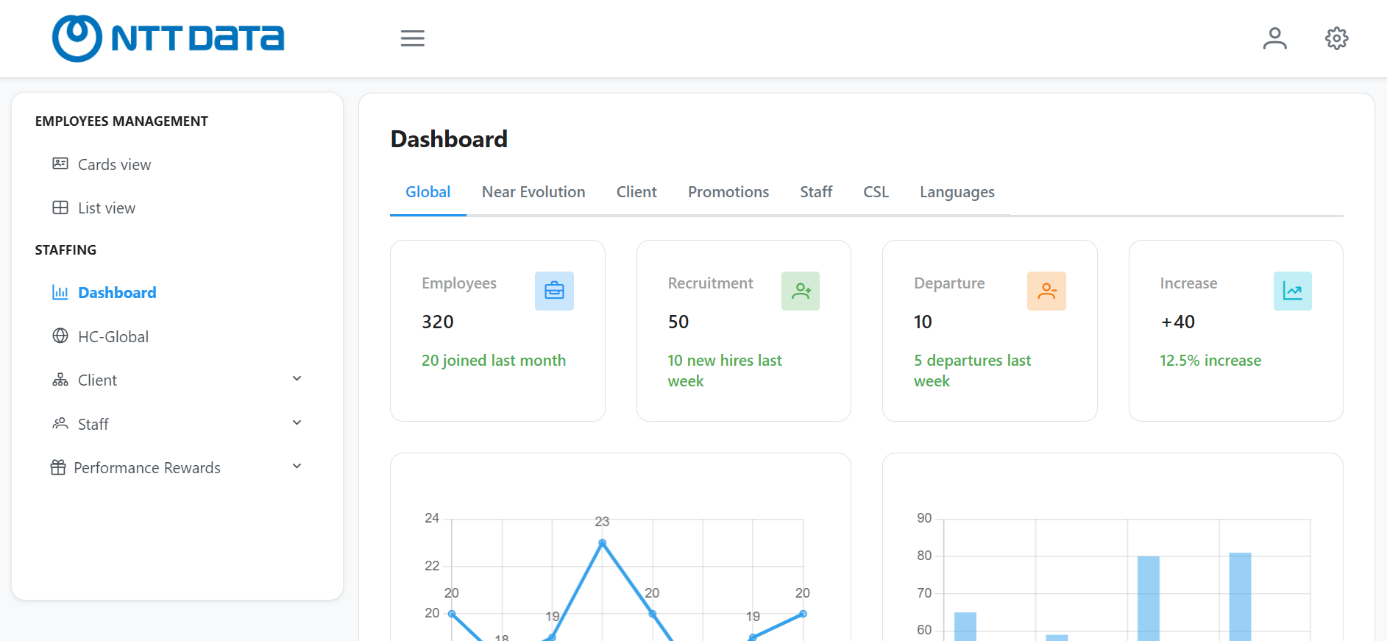
\includegraphics[width=150mm]{Image/dashboard}
		\caption{Dashboard}
		\label{fig:Dashboard}
	\end{figure}

	Those ones are interactive and allow custom requests

	
	\begin{figure}[H]
		\centering
		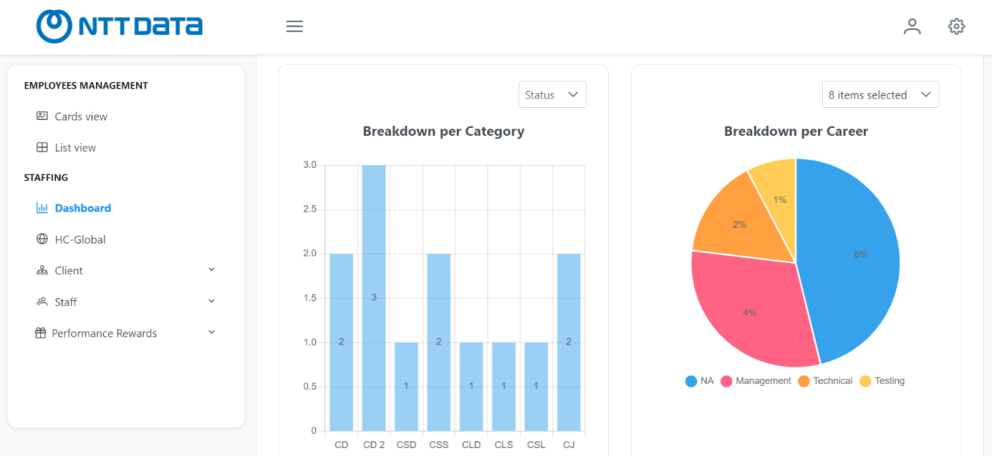
\includegraphics[width=150mm]{Image/dashboard2}
		\caption{Dashboard 2}
		\label{fig:Dashboard 2}
	\end{figure}

	\subsection{Employees}
	
	It is possible to have a quick summarize about all the employees
	\begin{figure}[H]
		\centering
		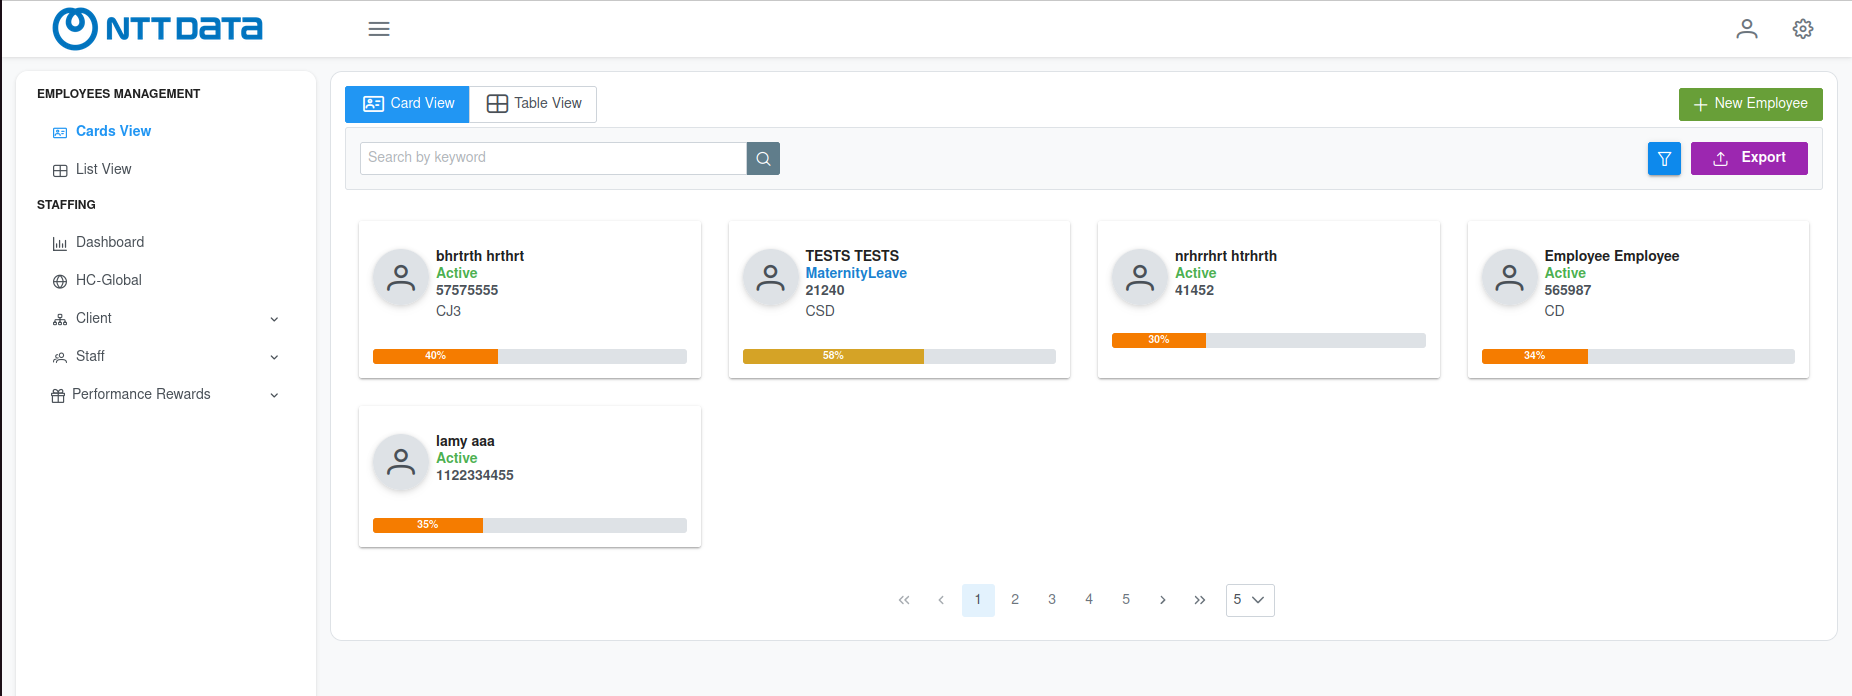
\includegraphics[width=150mm]{Image/cardview}
		\caption{Card view}
		\label{fig:Card view}
	\end{figure}

	But we can also have more details about them
	\begin{figure}[H]
		\centering
		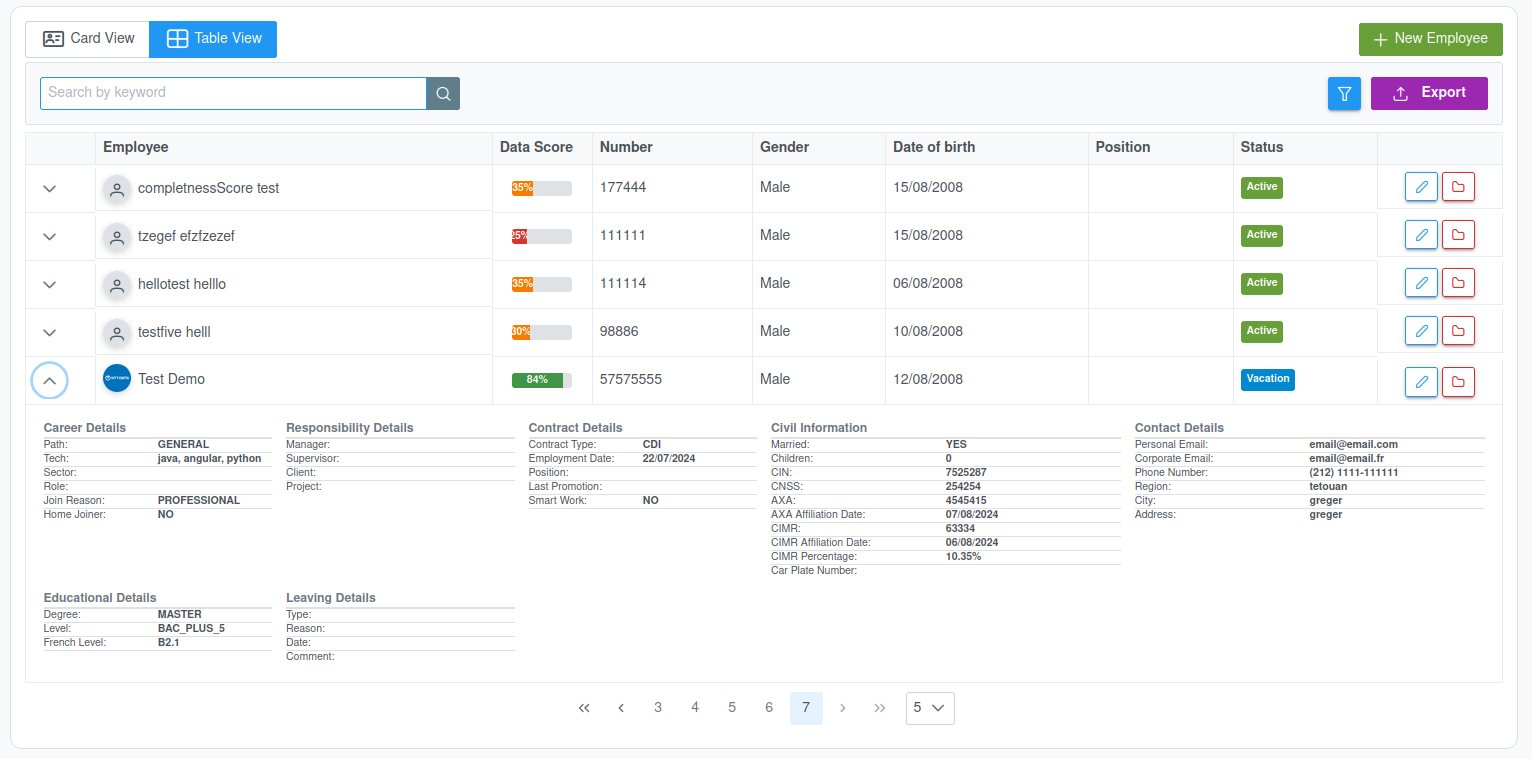
\includegraphics[width=150mm]{Image/tableview}
		\caption{Table view}
		\label{fig:Table view}
	\end{figure}
		
	And when we want to search an employee among all of this one, we just need to use the search bar or the filter with multiple criteria
	\begin{figure}[H]
		\centering
		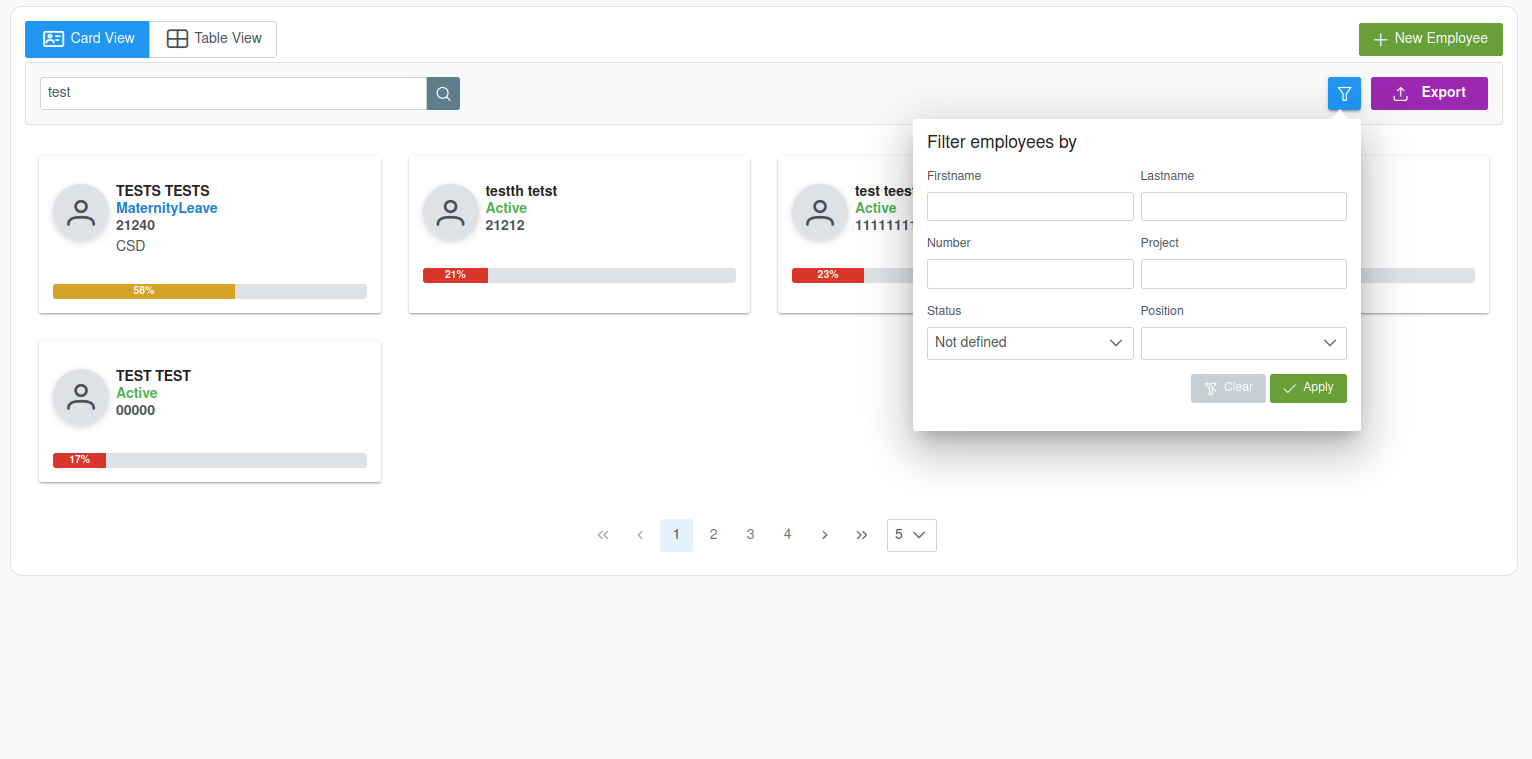
\includegraphics[width=150mm]{Image/search}
		\caption{Employee searching}
		\label{fig:Employee searching}
	\end{figure}

	But before to search or display them, we should first create them.
	For this we added the possibility to import data from an excel file, that can be done only by the admin with a direct request to the back-end (not part of the front-end application). For others, they can just create a new one by selecting the green button above:

	\begin{figure}[H]
	\centering
	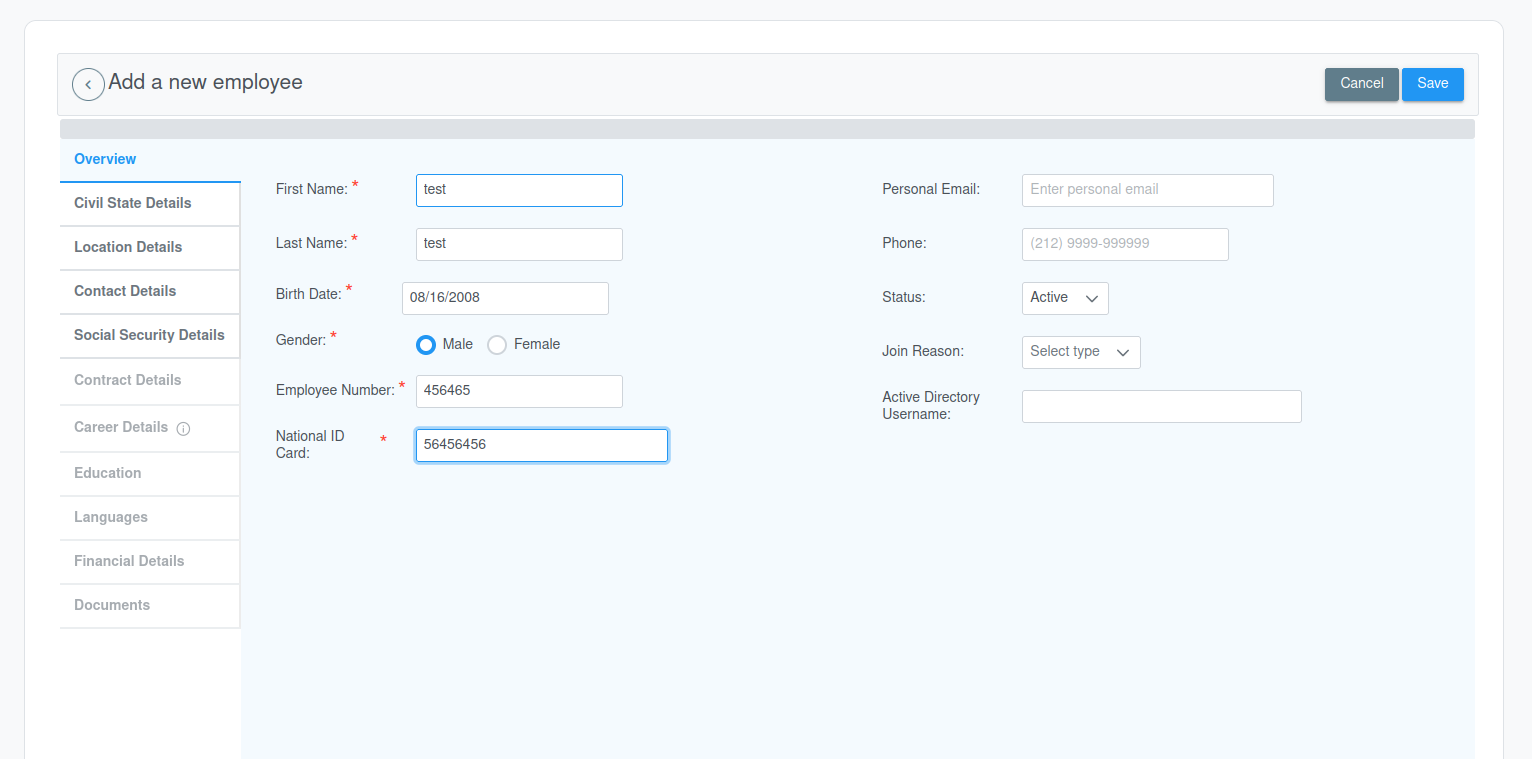
\includegraphics[width=150mm]{Image/employeeadd}
	\caption{Employee creation}
	\label{fig:Employee creation}
	\end{figure}
	
	We will need to fill at least the 6 required fields to create one.\\
	Then we can also update it:
	
	\begin{figure}[H]
	\centering
	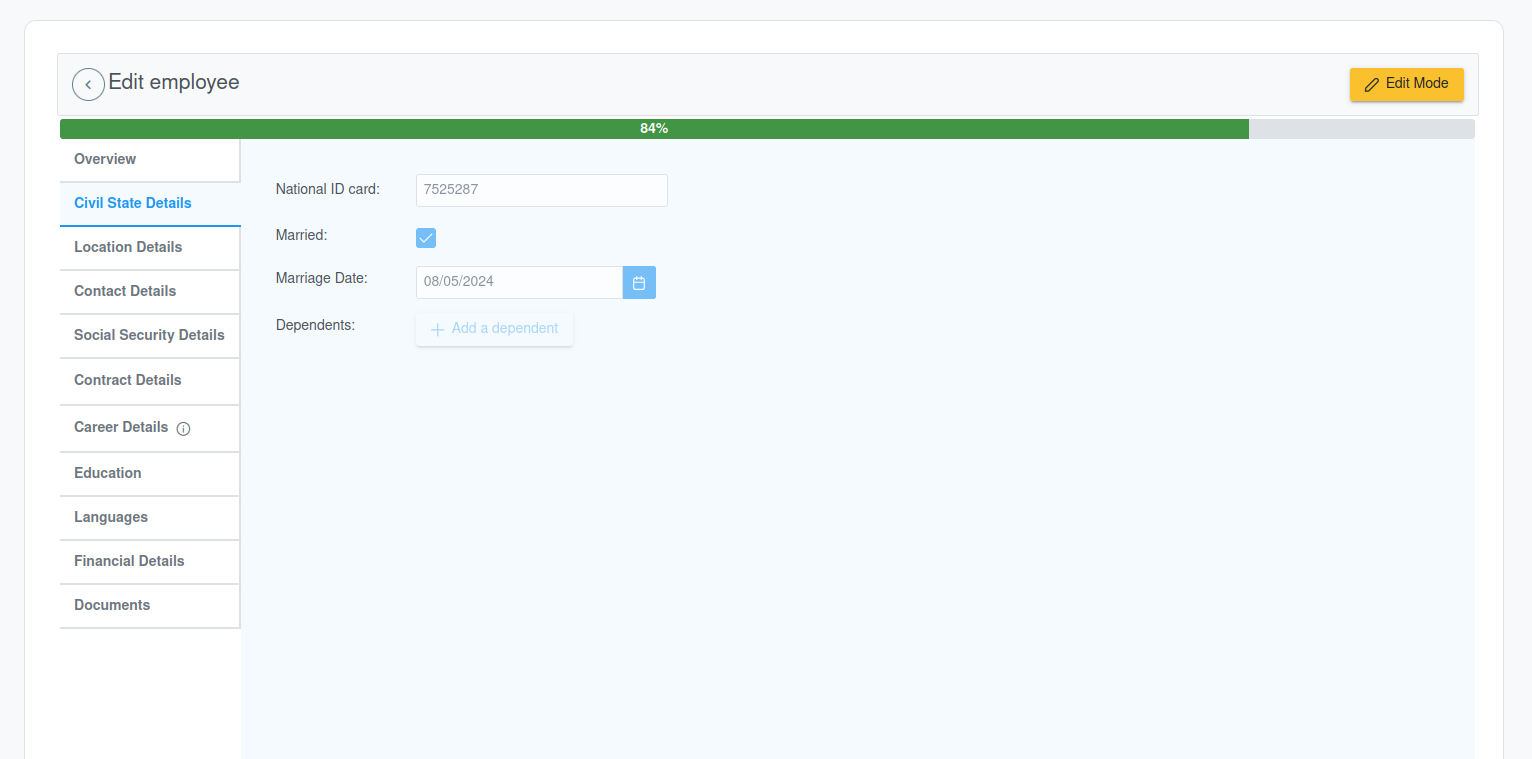
\includegraphics[width=150mm]{Image/employee1}
	\caption{Employee - 1}
	\label{fig:Employee - 1}
	\end{figure}

	We can then fill different information:
	
	\begin{figure}[H]
		\centering
		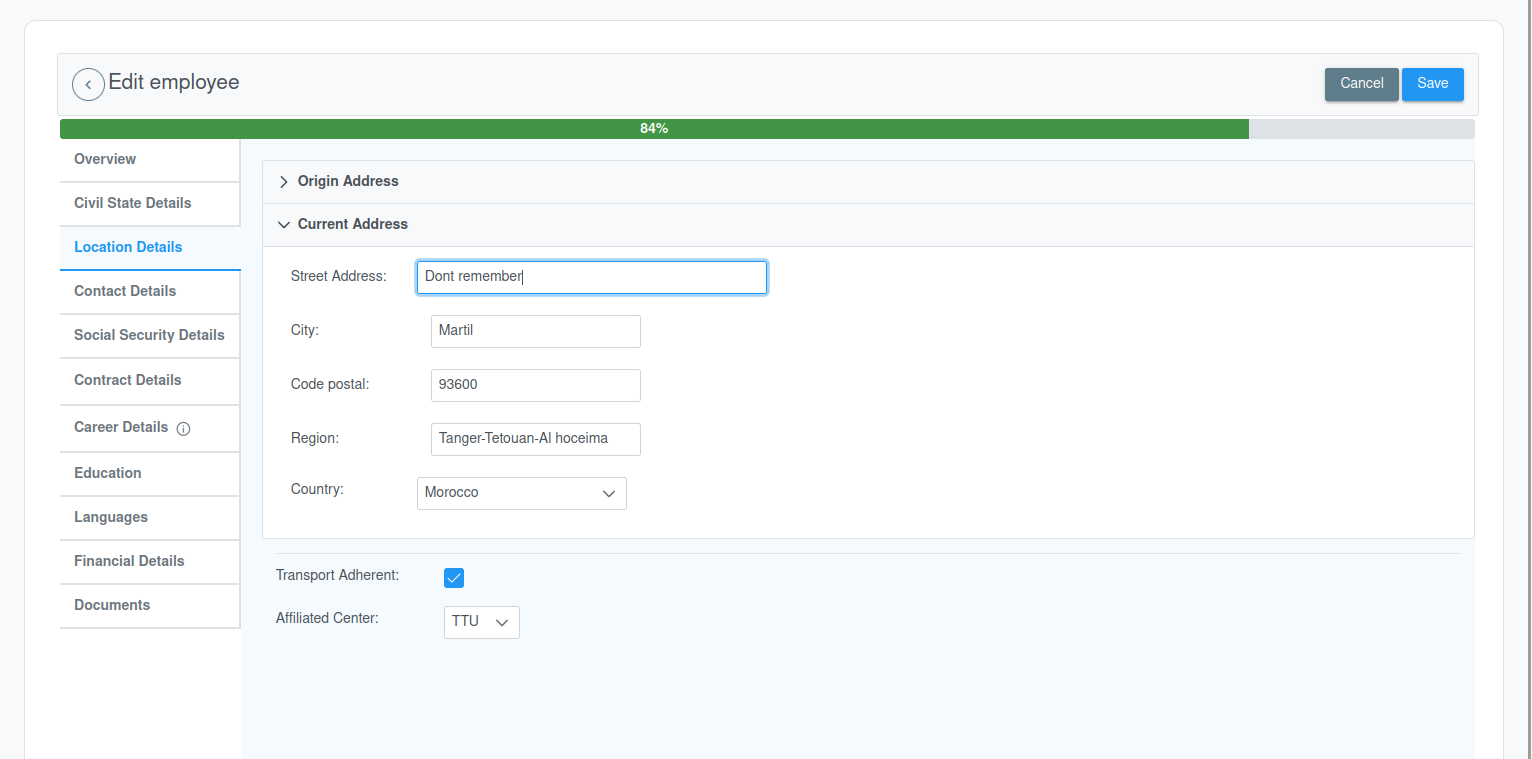
\includegraphics[width=150mm]{Image/employee2}
		\caption{Employee - 2}
		\label{fig:Employee - 2}
	\end{figure}
	
		
	\begin{figure}[H]
		\centering
		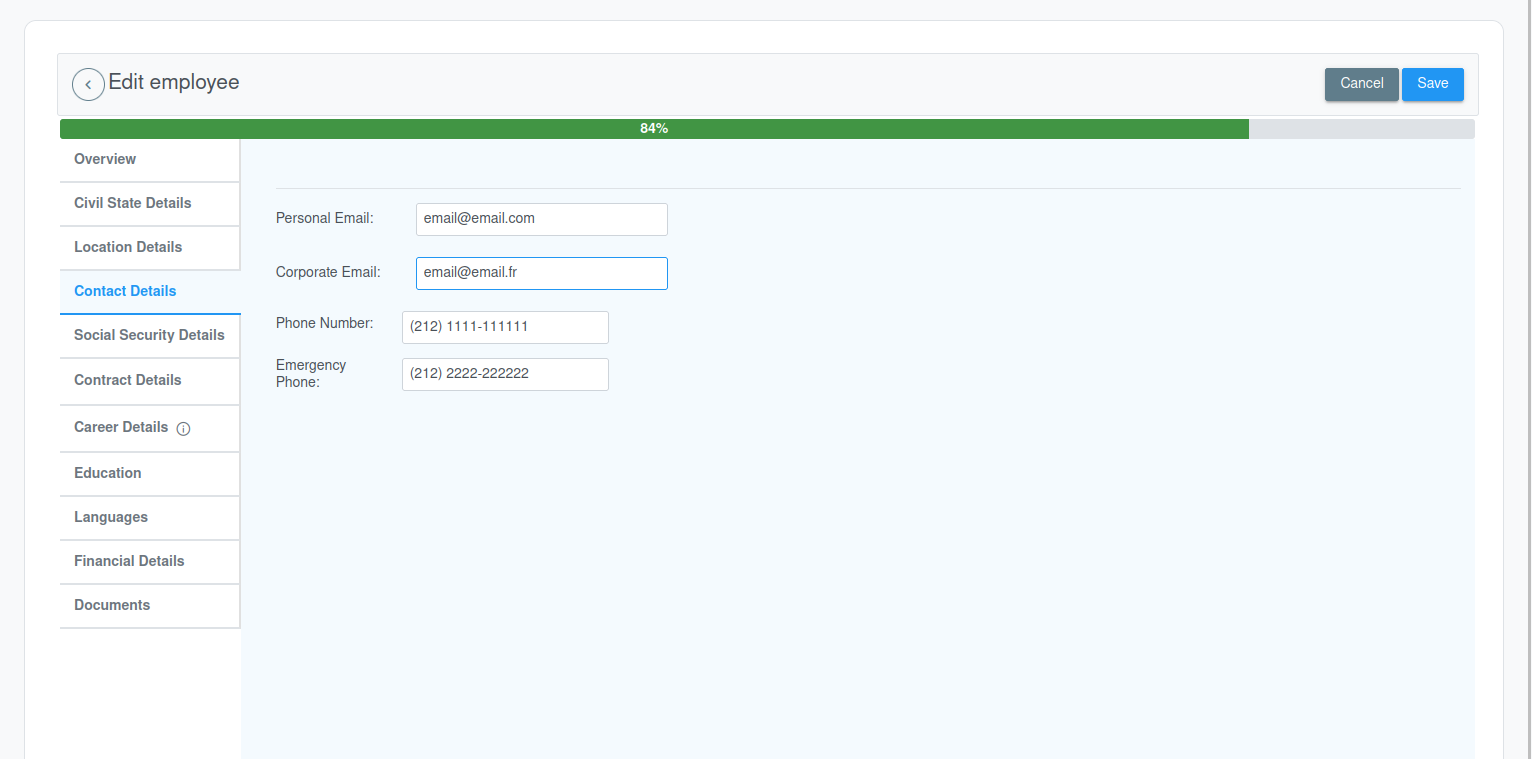
\includegraphics[width=150mm]{Image/employee3}
		\caption{Employee - 3}
		\label{fig:Employee - 3}
	\end{figure}
	
		
	\begin{figure}[H]
		\centering
		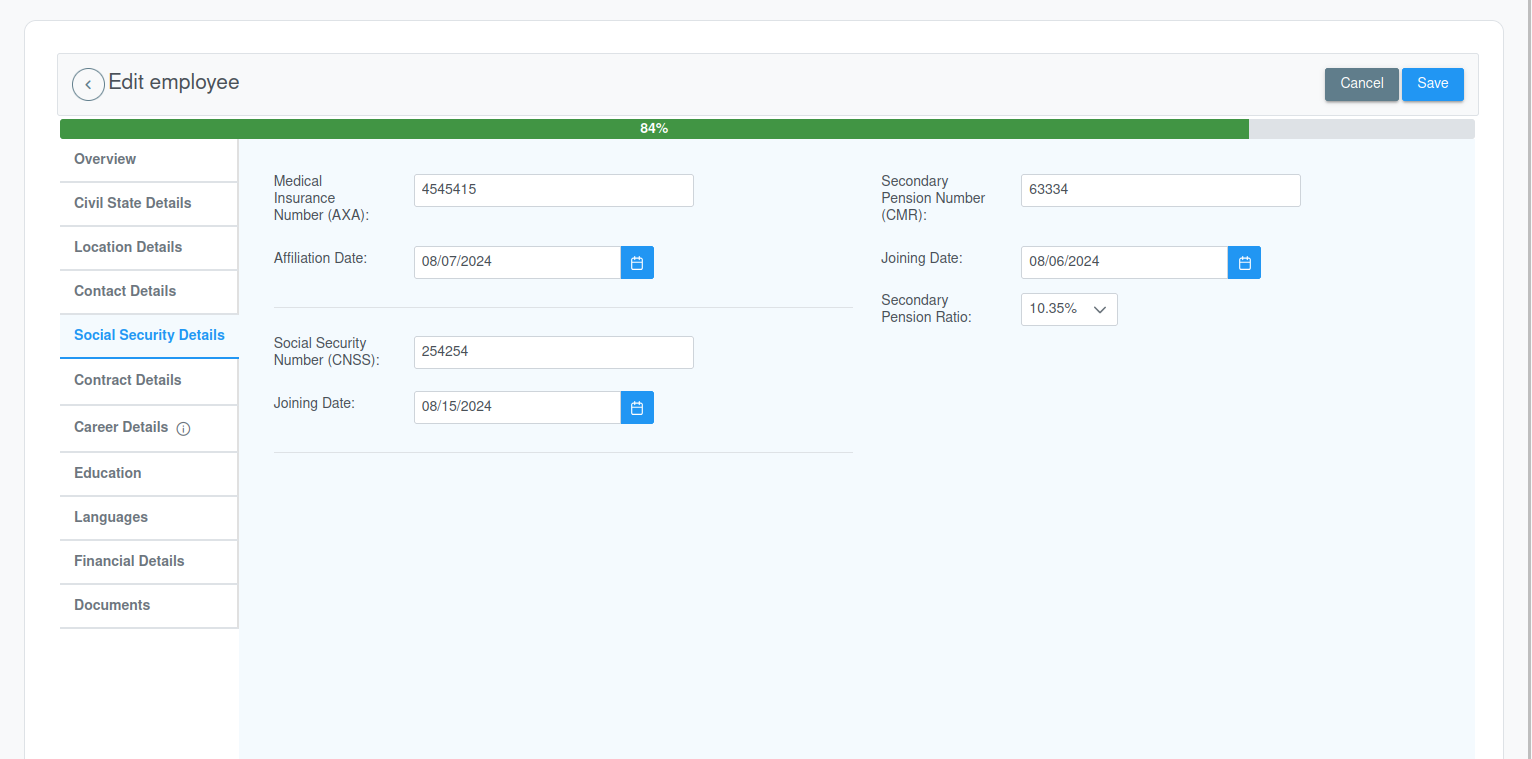
\includegraphics[width=150mm]{Image/employee4}
		\caption{Employee - 4}
		\label{fig:Employee - 4}
	\end{figure}
	
		
	\begin{figure}[H]
		\centering
		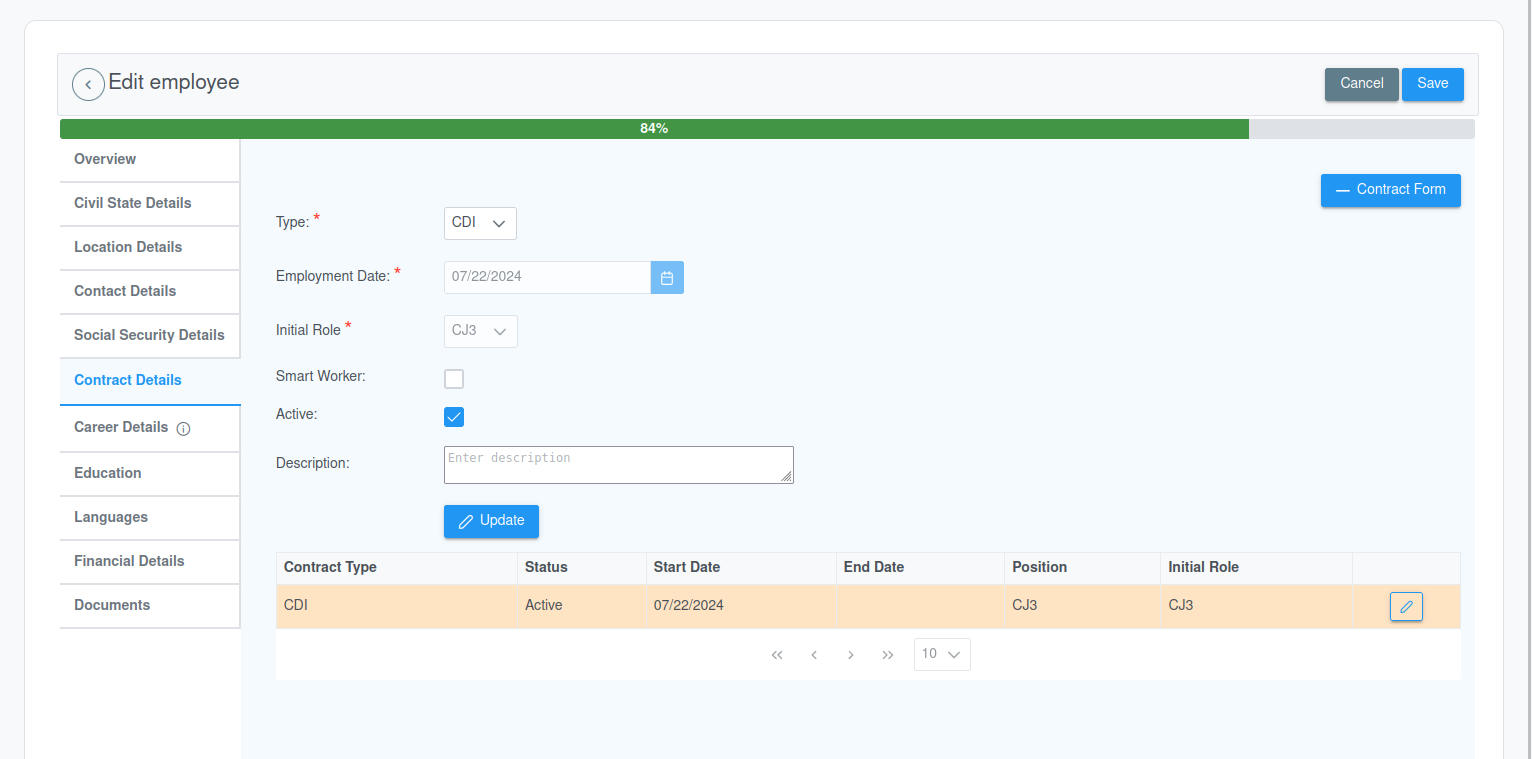
\includegraphics[width=150mm]{Image/employee5}
		\caption{Employee - 5}
		\label{fig:Employee - 5}
	\end{figure}
	
		
	\begin{figure}[H]
		\centering
		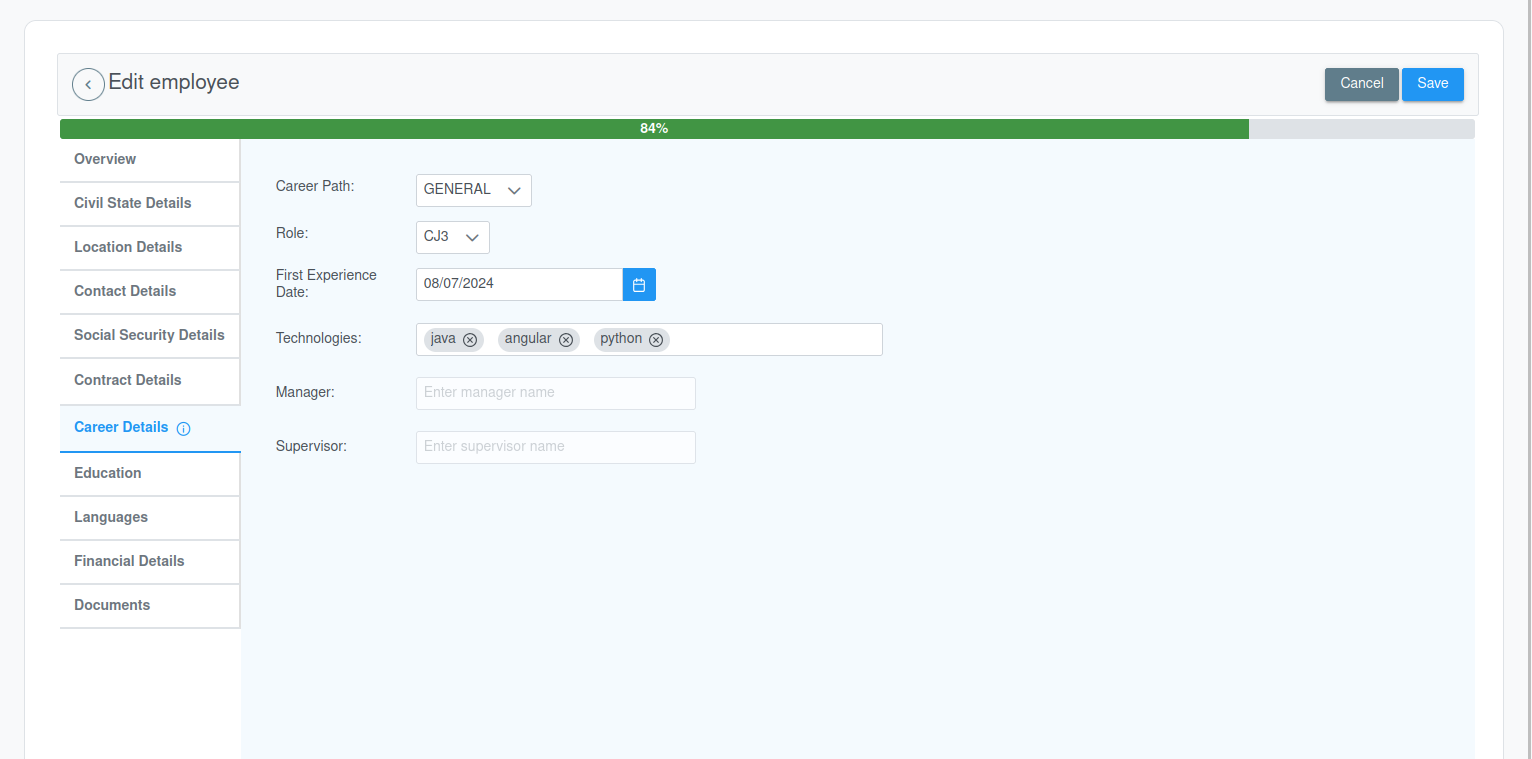
\includegraphics[width=150mm]{Image/employee6}
		\caption{Employee - 6}
		\label{fig:Employee - 6}
	\end{figure}
	
		
	\begin{figure}[H]
		\centering
		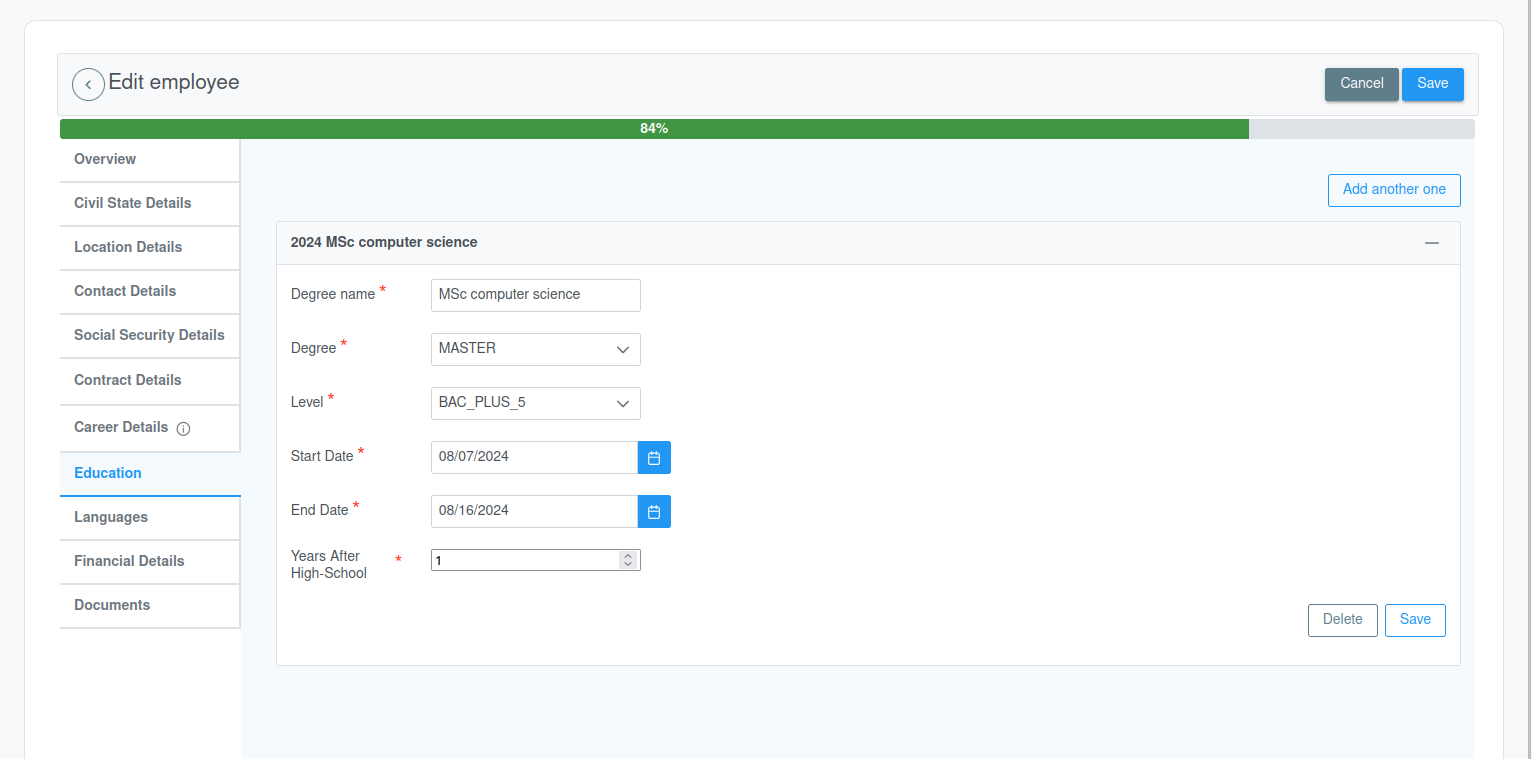
\includegraphics[width=150mm]{Image/employee7}
		\caption{Employee - 7}
		\label{fig:Employee - 7}
	\end{figure}
	
		
	\begin{figure}[H]
		\centering
		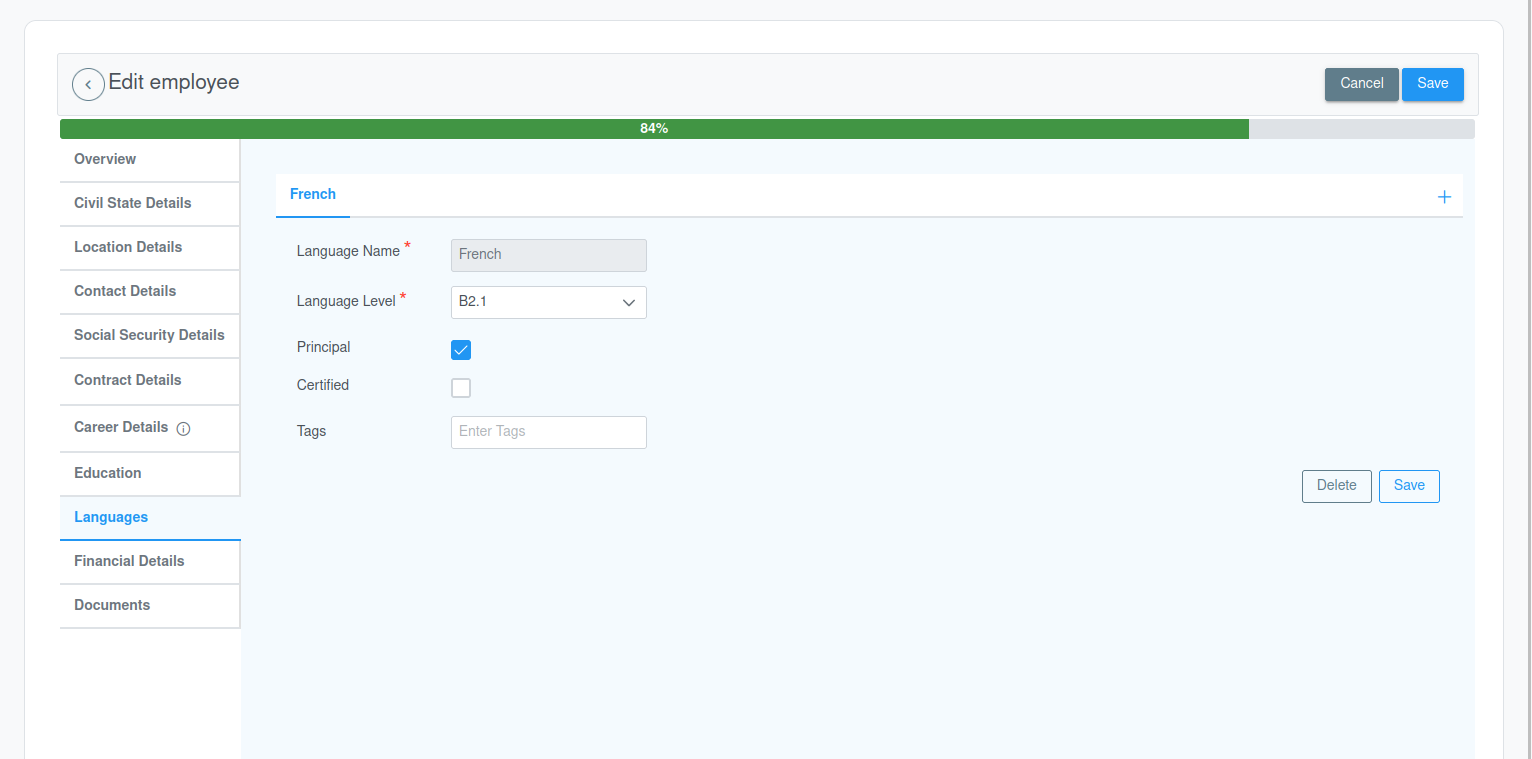
\includegraphics[width=150mm]{Image/employee8}
		\caption{Employee - 8}
		\label{fig:Employee - 8}
	\end{figure}
	
		
	\begin{figure}[H]
		\centering
		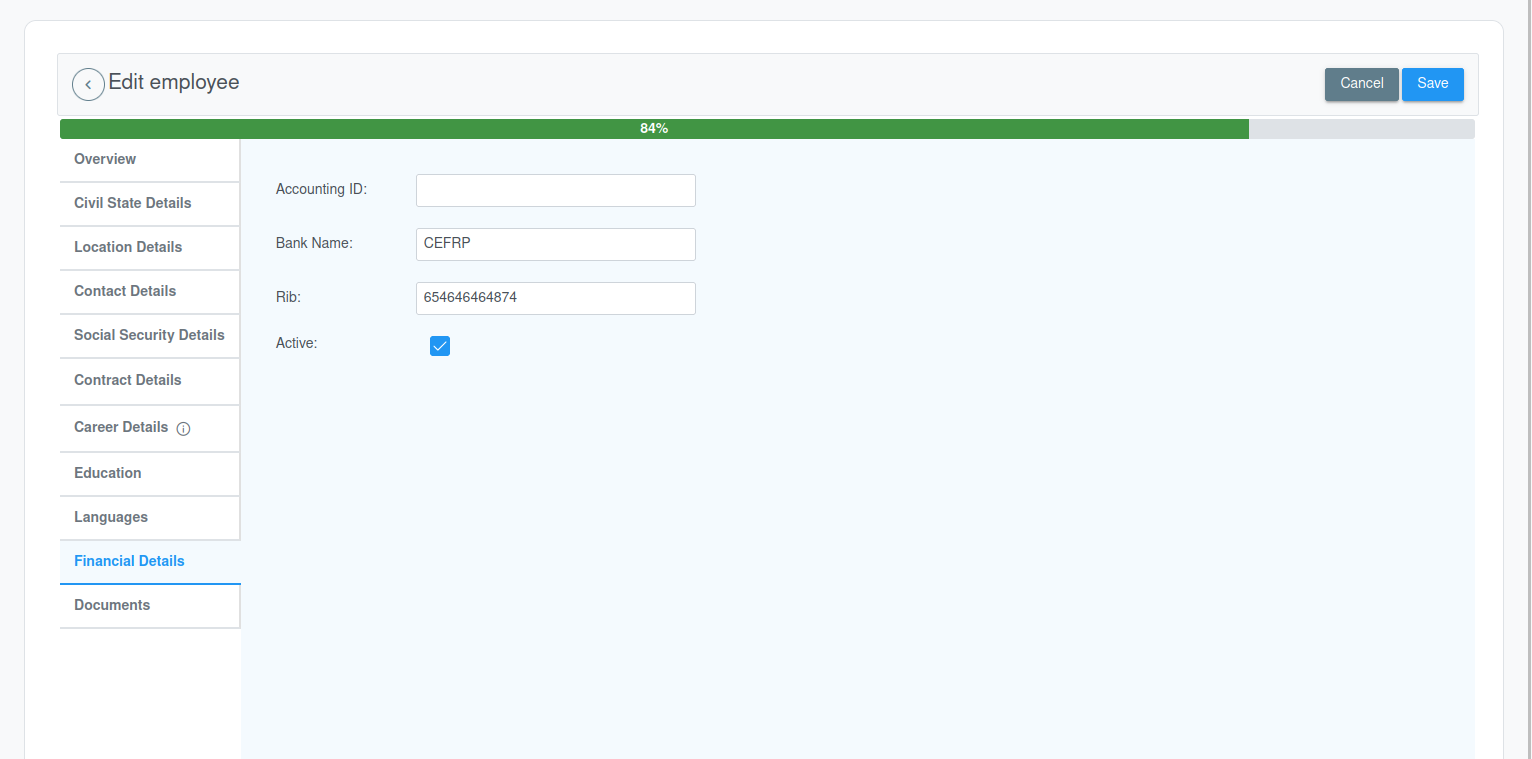
\includegraphics[width=150mm]{Image/employee9}
		\caption{Employee - 9}
		\label{fig:Employee - 9}
	\end{figure}
	
	Finally, we can upload different type of document
	\begin{figure}[H]
		\centering
		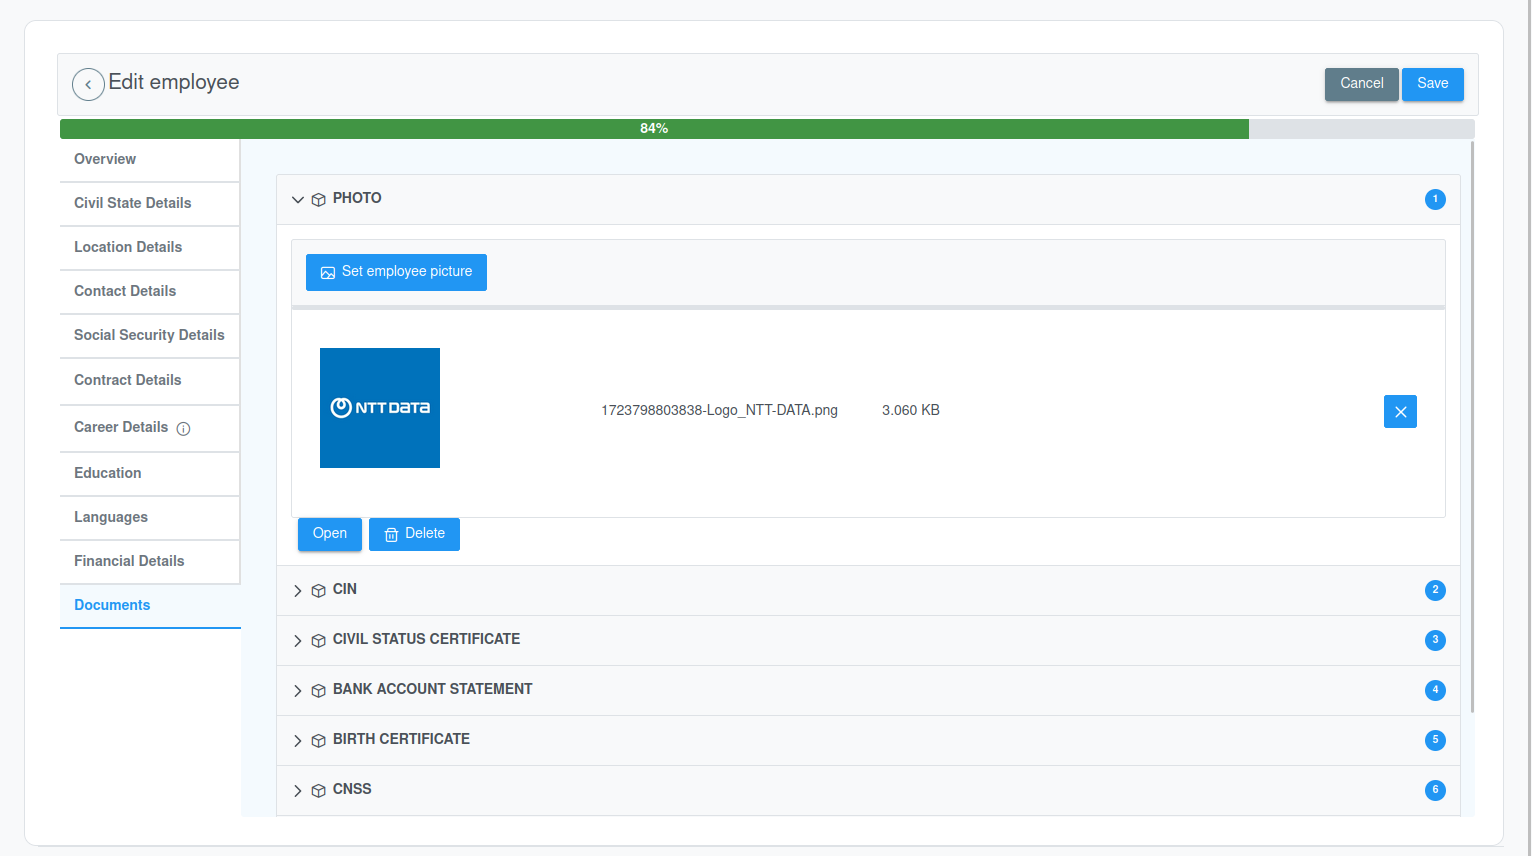
\includegraphics[width=150mm]{Image/employee10}
		\caption{Employee - 10}
		\label{fig:Employee - 10}
	\end{figure}

	
	\subsection{HC-Global}
	It is possible to display different statistics for each year, each month about employees of the company. This one also allows to export and import data
	
	\begin{figure}[H]
		\centering
		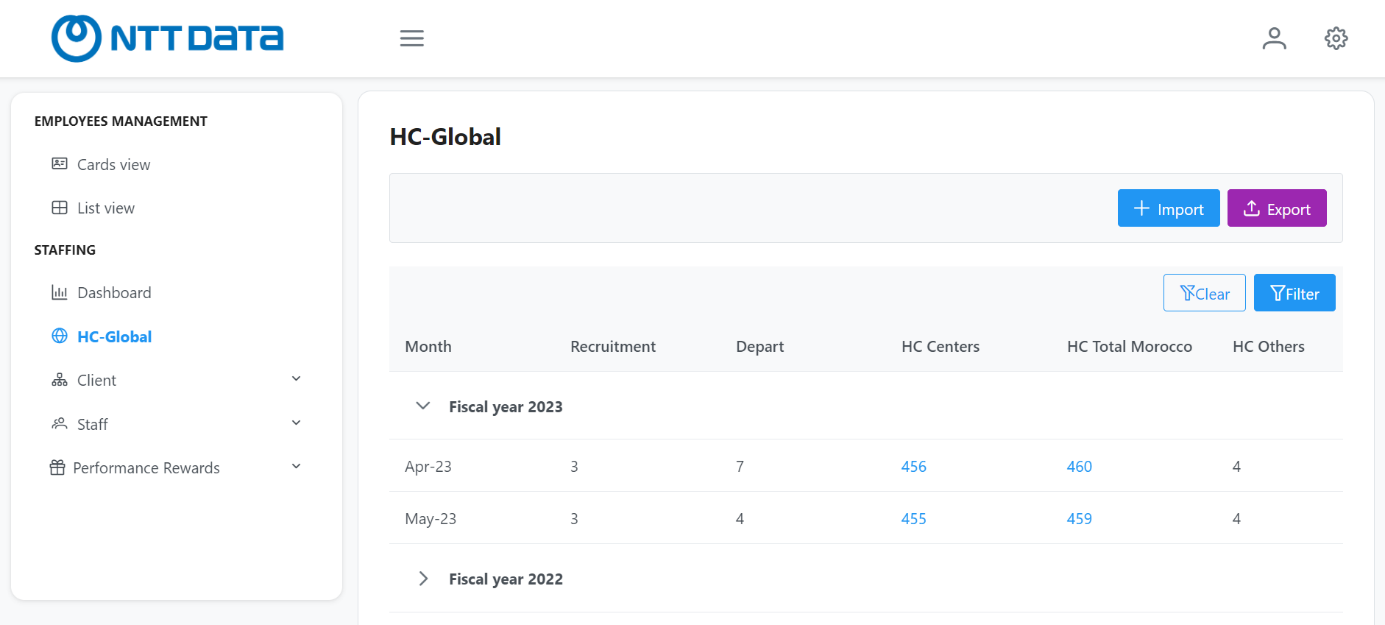
\includegraphics[width=150mm]{Image/hcglobal}
		\caption{HC-Global}
		\label{fig:HC-Global}
	\end{figure}


	\subsection{Client}
	We have the possibility to manage the client of the company
	
	\begin{figure}[H]
		\centering
		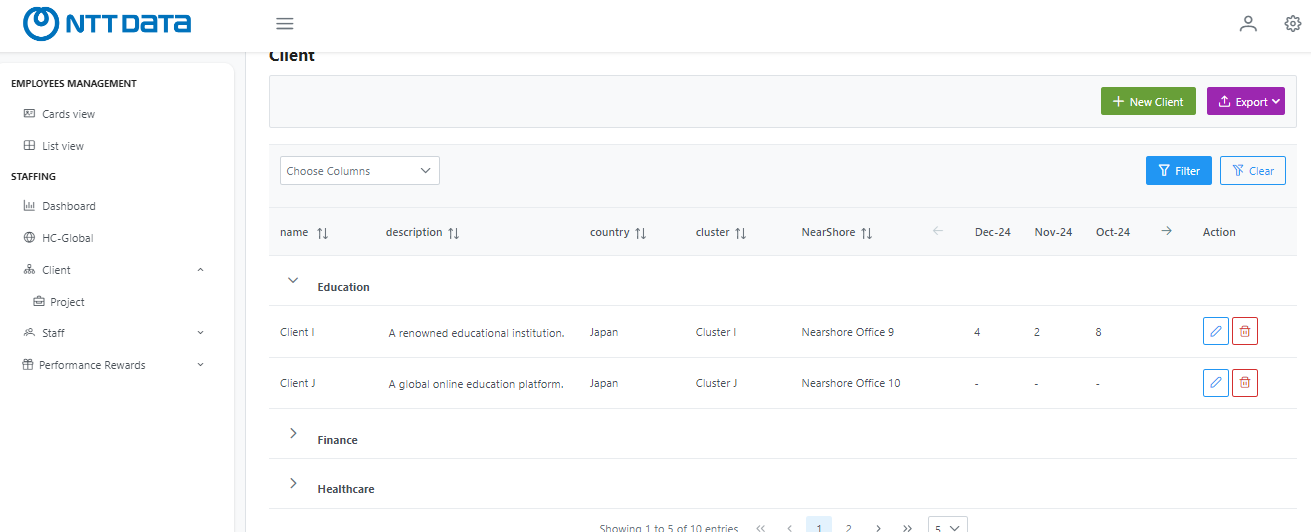
\includegraphics[width=150mm]{Image/clients}
		\caption{Clients}
		\label{fig:Clients}
	\end{figure}
	
	Creating a new one

	\begin{figure}[H]
		\centering
		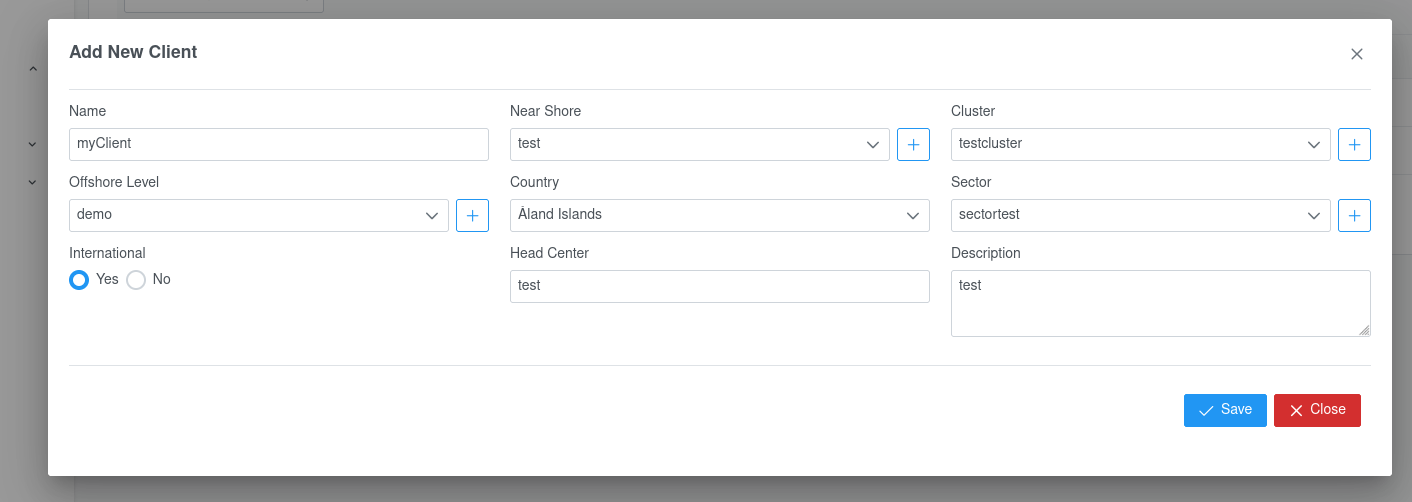
\includegraphics[width=150mm]{Image/clientadd}
		\caption{Create client}
		\label{fig:Create client}
	\end{figure}

	Then we assign a manager to the new client
	
	\begin{figure}[H]
		\centering
		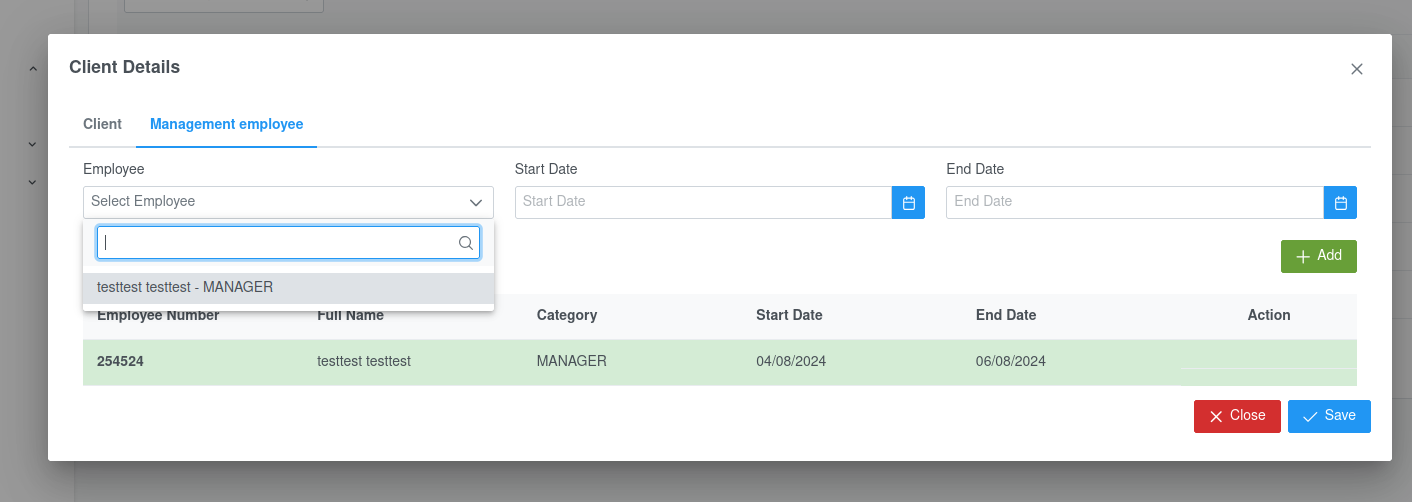
\includegraphics[width=150mm]{Image/clientassign}
		\caption{Asssign manager to client}
		\label{fig:Create client}
	\end{figure}

	Once done, we will need to create the project that the client is looking for
	\begin{figure}[H]
		\centering
		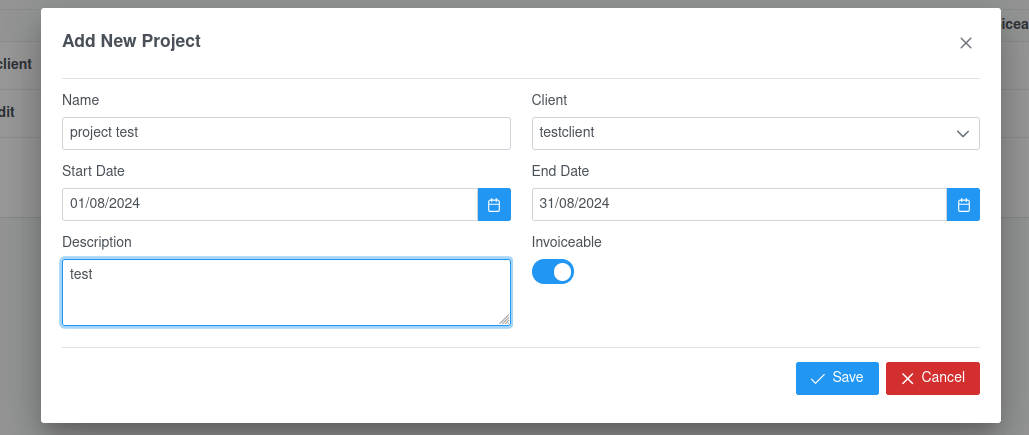
\includegraphics[width=150mm]{Image/projectadd}
		\caption{Create a project}
		\label{fig:Create a project}
	\end{figure}
	
	And then we might need employees to work on this one

	\begin{figure}[H]
		\centering
		\includegraphics[width=150mm]{Image/projectassign}
		\caption{Assign employee to a project}
		\label{fig:Assign employee to a project}
	\end{figure}

	\subsection{Staff}
	
	We have the possibility to display and manage all the current employees that have been assigned to a project
	
	\begin{figure}[H]
		\centering
		\includegraphics[width=150mm]{Image/staff}
		\caption{Display working employees}
		\label{fig:Display working employees}
	\end{figure}
	
	\subsection{Promotion}
	
	We also offer an interface to manage the promotion of the employees
	
	\begin{figure}[H]
		\centering
		\includegraphics[width=150mm]{Image/promotion}
		\caption{Promotions}
		\label{fig:Promotions}
	\end{figure}

	We can modify and update it
	\begin{figure}[H]
		\centering
		\includegraphics[width=150mm]{Image/promotiondetails}
		\caption{Promotions update}
		\label{fig:Promotions update}
	\end{figure}

	Then after we can validate, or not, the promotion

	\begin{figure}[H]
		\centering
		\includegraphics[width=150mm]{Image/promotionconfirm}
		\caption{Promotions confirmation}
		\label{fig:Promotions confirmation}
	\end{figure}

	We also keep a track of the interview
	\begin{figure}[H]
		\centering
		\includegraphics[width=150mm]{Image/promotioninterview}
		\caption{Interview}
		\label{fig:Interview}
	\end{figure}


	\section{Performance Rewards}
	
	Here we display the objectives of the different years
	\begin{figure}[H]
		\centering
		\includegraphics[width=150mm]{Image/performance}
		\caption{Performances}
		\label{fig:Performances}
	\end{figure}

	And visualize the performances
	\begin{figure}[H]
		\centering
		\includegraphics[width=150mm]{Image/performancegraph}
		\caption{Performance graph}
		\label{fig:Performance graph}
	\end{figure}

	\section{Configuration}
	
	Specific users, also have access to different information, configuration. Here we can display the increasing
	\begin{figure}[H]
		\centering
		\includegraphics[width=150mm]{Image/conf}
		\caption{Configuration}
		\label{fig:Configuration}
	\end{figure}

	We can also define the range of wages for all positions
	\begin{figure}[H]
	\centering
	\includegraphics[width=150mm]{Image/confband}
	\caption{Configuration wages}
	\label{fig:Configuration wages}
	\end{figure}


	\newpage
	\section{Conclusion}

	Employee management is a crucial component of any business. It is not just an administrative task but a key element of corporate strategy. Employees are the heart of any organization, and effective management is crucial for productivity and success. \\
	This system, primarily designed for the human resources and staffing team, automates tasks related to employee management such as recruitment, performance tracking, document management as well as client management, their projects, and their employees assigned.\\
	
	Our application has successfully automated and normalized many tasks and improved the efficiency of employee management within the company. However, we also acknowledge aspects that need improvement and challenges to be addressed.\\
	
	This immersion in the company, provided me with a concrete and enriching perspective on the dynamics of IT projects. I have fully grasped the crucial importance of collaboration and teamwork in achieving ambitious projects. Similarly, I have been able to assess the significant impact of modern technologies on optimizing processes and improving operational efficiency.\\
	
	This experience will serve as a real springboard for my professional development. The technical skills acquired are undeniable, but as valuable as the professional lessons taught, equipping me with a more comprehensive and pragmatic vision to tackle future challenges with confidence and determination.
	

	\newpage
	\section{Glossary}

\textbf{API:} Application Programming Interface. A set of rules and definitions that allows different software applications to communicate with each other.\\

\textbf{AWS:} Amazon Web Services. A comprehensive cloud platform offering various services such as computing power, storage, and networking.\\

\textbf{Back-end:} The server-side part of an application that handles business logic, database interactions, and server communication.\\

\textbf{Branch:} In version control systems, a branch is an independent line of development that allows multiple developers to work on different features simultaneously.\\

\textbf{CI/CD:} Continuous Integration/Continuous Deployment. Practices in software engineering that ensure automated testing, integration, and deployment of applications.\\

\textbf{Command execution:} The process of running a specific command to directly order the OS in an operating system or application environment.\\

\textbf{CPU:} Central Processing Unit. The primary component of a computer that performs most of the processing inside a computer.\\

\textbf{CRUD:} Acronym for Create, Read, Update, Delete. It represents the four basic operations of persistent storage in database management systems and software applications.

\textbf{CSS:} Cascading Style Sheets. A style sheet language used to describe the presentation and design of a document written in HTML or XML.\\

\textbf{Database:} An organized collection of data, typically stored electronically in a structured format.\\

\textbf{DBMS:} Database Management System. Software that interacts with databases to manage and query data.\\

\textbf{Design pattern:} A general, reusable solution to a commonly occurring problem within a given context in software design.\\

\textbf{Docker:} An open-source platform that automates the deployment of applications inside lightweight, portable containers.\\

\textbf{DTO:} Data Transfer Object. A design pattern used to transfer data between software application subsystems.\\

\textbf{Elastic Search:} A distributed search and analytics engine commonly used for indexing large volumes of data and for text search.\\

\textbf{Environments:} Different setups or configurations where software applications are developed, tested, and deployed (e.g., development, local, production).\\

\textbf{Filters:} In Spring Security, filters are mechanisms used to process requests and responses within the web application security framework. They are used to perform tasks such as authentication, authorization, logging, and data transformation based on specific criteria. Filters are part of the request processing chain and can modify or inspect requests and responses before they reach the application or after they leave it.\\

\textbf{Frameworks:} Predefined structures or platforms for developing software applications that provide reusable code and tools.\\

\textbf{Front-end:} The client-side part of an application that deals with the user interface and user experience (UI/UX).\\

\textbf{Heroku:} A cloud platform that enables developers to build, run, and scale applications quickly without managing infrastructure.\\

\textbf{HTML:} Hyper Text Markup Language. The standard language used to create web pages and web applications.\\

\textbf{IDE:} Integrated Development Environment. Software providing comprehensive tools (e.g., code editor, debugger) for developers to write and test code.\\

\textbf{JSON:} JavaScript Object Notation. A lightweight data-interchange format used for storing and exchanging structured data.\\

\textbf{Libraries:} Sets of code that developers can use to optimize and simplify tasks in software development.\\

\textbf{Minio:} An open-source, high-performance object storage system compatible with Amazon S3.\\

\textbf{MVC:} Model-View-Controller. A software architectural pattern for implementing user interfaces by separating concerns into three interconnected components: Model, View, and Controller.\\

\textbf{NPM:} Node Package Manager. A package manager for JavaScript, used to install libraries and manage dependencies in Node.js applications.\\

\textbf{OPA:} Open Policy Agent. A general-purpose policy engine that enables fine-grained access control across systems.\\

\textbf{Operating System (OS):} The software that manages hardware resources and provides services for computer programs.\\

\textbf{Policies:} Rules or guidelines applied in software systems to control access, security, and operations.\\

\textbf{POC:} Proof of Concept. A prototype or demonstration used to verify a concept or idea in a project.\\

\textbf{PostgreSQL:} An open-source relational database management system (RDBMS) known for its extensibility and standards compliance.\\

\textbf{Processing:} The act of executing tasks or computations on data by a computer's CPU.\\

\textbf{PR:} Pull Request, a request to bring changes in the source code of the project.

\textbf{RAM:} Random Access Memory. A type of computer memory that stores data temporarily, allowing for fast read and write operations.\\

\textbf{Token:} A digital object used to authenticate and authorize users in secure communication, often used in token-based authentication systems (e.g., JWT).\\

\textbf{TS:} TypeScript. A strongly typed programming language that builds on JavaScript, offering better tooling for large applications.\\

\textbf{Mock:}
\textbf{Beans:}
\textbf{UI:}
\textbf{DOM}
\textbf{dependencie}
	
	\newpage
	\section{Références bibliographiques}
\bibliographystyle{plain}
\bibliography{biblio}  

\citep{JPATABLE}
% https://docs.spring.io/spring-data/jpa/docs/current/api/org/springframework/data/jpa/repository/JpaRepository.html
% https://www.baeldung.com/spring-data-jpa-find-by-vs-find-all-by
% https://www.geeksforgeeks.org/spring-data-jpa-query-annotation-with-example/
% https://docs.spring.io/spring-data/jpa/reference/jpa/query-methods.html
% table strategy: https://www.javatpoint.com/jpa-single-table-strategy

%	\newpage	
%	\section{Annexe}


\end{document}